\documentclass[11pt]{article}
\usepackage{geometry}
\usepackage{graphicx}
\usepackage{wrapfig}
\usepackage{float}
\usepackage{fancyvrb}
\usepackage{caption}
\usepackage{subcaption}
\usepackage[T1]{fontenc}
\usepackage[utf8]{inputenc}
\usepackage{helvet}
\usepackage[table]{xcolor}
\renewcommand{\familydefault}{\sfdefault}
%\usepackage{titlesec}
%\titlespacing\section{1pt}{12pt plus 2pt minus 2pt}{1pt plus 2pt minus 2pt}
%\titlespacing\subsection{1pt}{12pt plus 2pt minus 2pt}{pt plus 2pt minus 2pt}
%\titlespacing\subsubsection{5pt}{12pt plus 2pt minus 2pt}{1pt plus 2pt minus 2pt}
%\usepackage{float}
\usepackage{booktabs}
\usepackage[hidelinks]{hyperref}
\usepackage{hyperref}
\usepackage{float}
\hypersetup{
	colorlinks=true,
	linkcolor=blue,
	filecolor=magenta,      
	urlcolor=cyan,
	pdftitle={Overleaf Example},
	pdfpagemode=FullScreen,
}
\setcounter{tocdepth}{4}
\urlstyle{same}
\geometry{margin=0.5in}
%opening
%\titleformat*{\section}{\small\bfseries}
\bibliographystyle{unsrt}
\author{Ethan Holleman}
\title{Variable region insert design and cloning strategies}

\begin{document}

\maketitle
%\begin{abstract}
%	Abstract text here
%\end{abstract}

\tableofcontents
\pagebreak

\section{Background}

R-loops are prevalent, functionally important, non-B DNA structures that form co-transcriptionally when the nascent RNA strand hybridizes back to the DNA template forming a DNA-RNA hybrid \cite{chedin_nascent_2016}. R-loops are formed ubiquitously across the genomes of all organisms often occupying large fractions of the genomes in a cell population. 

\begin{figure}[H]
	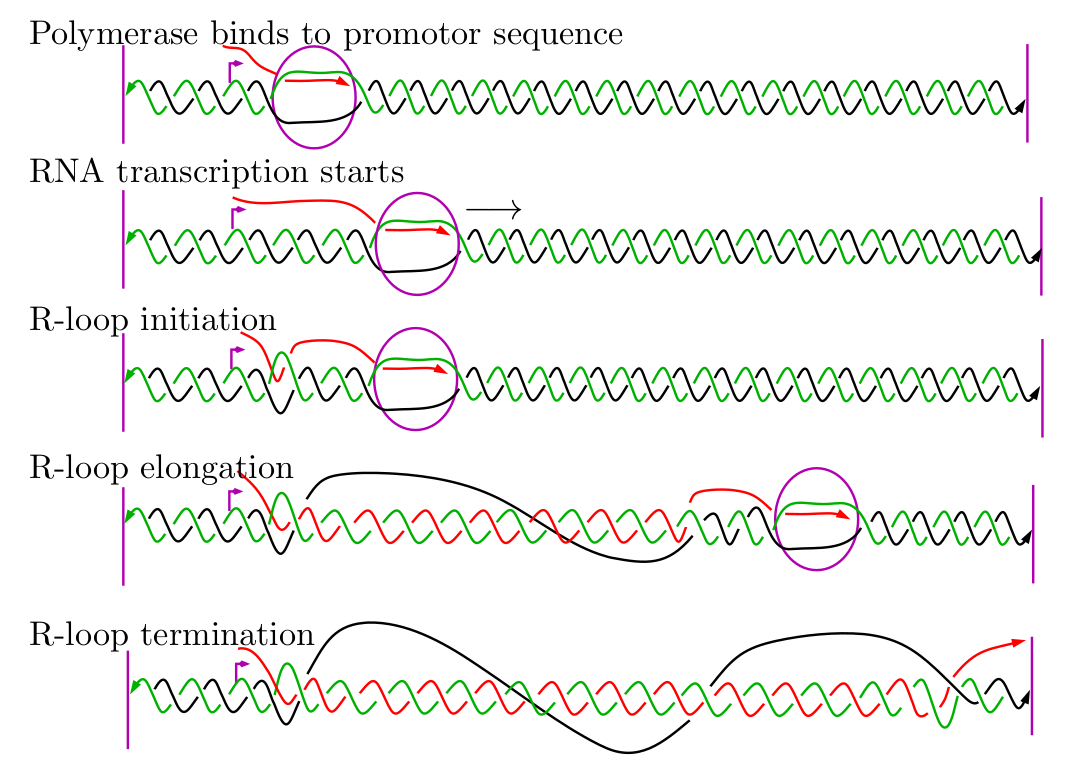
\includegraphics[width=12cm]{images/r-loops/rloop_stages.png}
	\centering
	\caption{Stages of R-loop formation. The encircled region represents the transcription bubble. The polymerase moves from left to right, starting at the promoter region (purple arrow). The upper strand (in red) in the bubble corresponds to the nascent RNA transcript, generated in the 5' to 3' direction. The R-loop initiates in frame 3, elongates in frame 4, and terminates in frame 5. Vazquez, Chedin and Natasa, 2020.}
	\label{fig:1}
\end{figure}

R-loops have been shown to cover approximately 5\% of the human genome, and generally, their formation is favored by regions with high GC skew (overabundance of G over C nucleotides) and GC content (percentage of G and C nucleotides) as the potential DNA-RNA hybrids formed over these sequences tend to be more energetically favorable with respect to R-loop formation\cite{Stolz2019}. Beyond these broad associations there has been little investigation into the specific sequence characteristics that influence R-loop initiation and termination, representing a significant gap in knowledge that continues to become increasingly pressing as the recognized scope of these structure's impact on cellular functions continues to grow. Here, I describe a detailed strategy for the systematic investigation of the impact of DNA sequence on R-loop initiation and termination which seeks to implement the methods described by Vazquez, Chedin and Natasa in NSF proposal number 2054347. 


\section{Insert design}

The overall goal of this series of experiments is to transcribe carefully controlled DNA sequences, referred to as inserts, in order to systematically observe the effects of these controlled sequences on R-loop initiation and termination \emph{in vitro}. Inserts are composed of two types of DNA components; the variable and infrastructure regions. The variable region is the sequence of interest with respect to R-loop formation while infrastructure sequences are additional nucleotide blocks that allow for the insertion of variable regions into specific plasmid backbones in a modular fashion. The distinct regions that compose each insert are described below. 

\begin{figure}[H]
	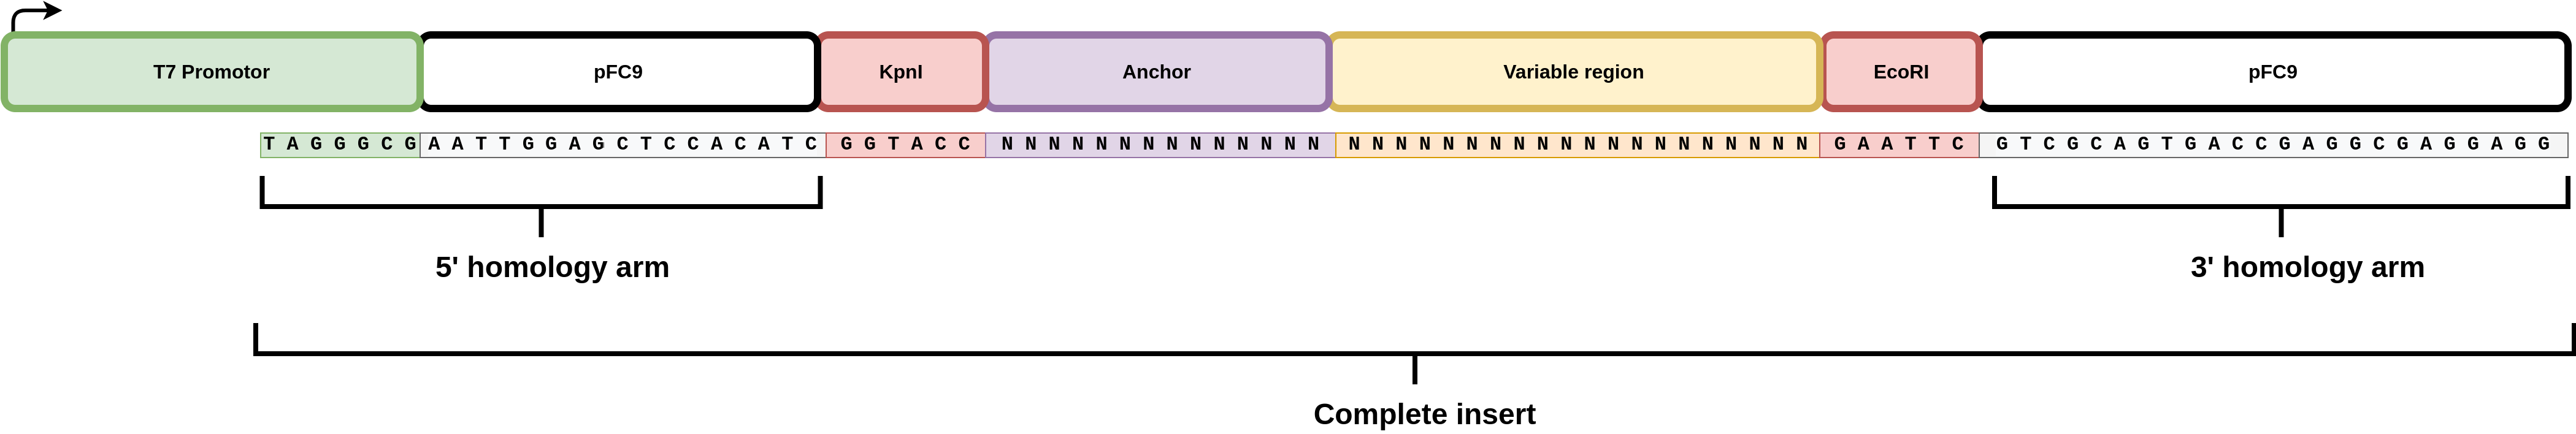
\includegraphics[width=16cm]{images/variable_region/construct_diagrams-Detailed-Insert.png}
	\centering
	\caption{Diagram of a complete insert. Colored boxes represent features insert sequences are derived from while colored sequences represent the actual nucleotide sequence.}
	\label{figure:1}
\end{figure}


\subsection{5' homology arm and KpnI recognition site}

The first 30 bp of each insert will be composed of the 5' homology arm and a KpnI recognition site. These sequences are included to facilitate Gibson and restriction enzyme cloning into pFC9 and pFC8 respectively. These 30 bp are taken directly from nucleotides 27 - 56 of pFC9.

\begin{figure}[h]
	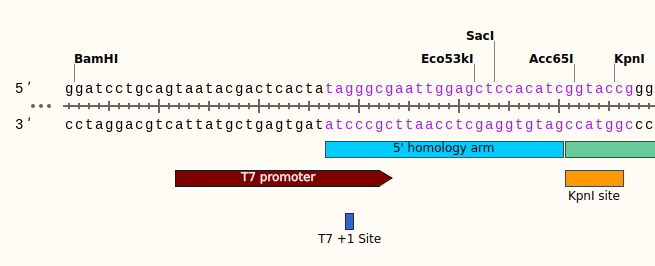
\includegraphics[width=12cm]{images/variable_region/5_homology_arm.png}
	\centering
	\caption{Location in pFC9 from which the 5' homology arm and KpnI site are modeled after. The entire 30 bp sequence is shown in purple with the 5' homology arm highlighted as a feature in blue and the KnpI site in orange.}
	\label{fig:homology_5}
\end{figure}

This strategy will mean recognition sites for Eco53KI, SacI and Acc65I will be included in the 5' homology arms. However, none of these enzymes will be utilized in any cloning protocols and so only the KpnI site is noted in diagrams.


\subsubsection{Anchor region}

The anchor region serves as a constant 15 nucleotide sequence that is always present in any final assembled construct adjacent to the 5' end of the variable region. This region provides significant utility when attempting to clone inserts already present in a plasmid into an alternative backbone. As long as the anchor region is present and intact, the number of primers required to amplify the insert region will not be dependent on the number of variable regions but the number of unique backbones. This utility is more explicitly shown in sections \ref{sec:tac-init} and \ref{sec:tac-termination}. 

Since this region is intended to be used as part of a PCR primer it was selected from candidate random sequences that satisfied the requirements below.

\begin{itemize}
	\item Does not contain any common sub-strings of minimum length equal to 75\% of the anchor's own length with any variable region or plasmid backbone.
	\item Does not contain the recognition sites for any restriction enzyme used in any relevant cloning procedure (see table \ref{tab:enzymes}).
	\item Does not contain single stretches of single nucleotides greater than three nucleotides in length.
\end{itemize}


\subsubsection{Variable regions}

Each insert will contain 1 variable region designed to test the effects of different sequence properties, namely GC / AT skew, GC content and G / C clustering, on R-loop initiation and termination. Each variable region will be 200 bp in length and 31 different variable regions with the properties described in table \ref{table:1} will ultimately be synthesized. 

\begin{table}
	\centering
\begin{tabular}{lrrrl}
	\toprule
	name &  GC skew &  GC content &  AT skew & G cluster length \\
	\midrule
	VR-1 &      0.0 &         0.4 &      0.0 &             NA \\
	VR-2 &      0.0 &         0.5 &      0.0 &             NA \\
	VR-3 &      0.0 &         0.6 &      0.0 &             NA \\
	VR-4 &      0.0 &         0.7 &      0.0 &             NA \\
	VR-5 &      0.1 &         0.4 &      0.0 &             NA \\
	VR-6 &      0.1 &         0.5 &      0.0 &             NA \\
	VR-7 &      0.1 &         0.6 &      0.0 &             NA \\
	VR-8 &      0.1 &         0.7 &      0.0 &             NA \\
	VR-9 &      0.2 &         0.4 &      0.0 &             NA \\
	VR-10 &      0.2 &         0.5 &      0.0 &             NA \\
	VR-11 &      0.2 &         0.6 &      0.0 &             NA \\
	VR-12 &      0.2 &         0.7 &      0.0 &             NA \\
	VR-13 &      0.4 &         0.4 &      0.0 &             NA \\
	VR-14 &      0.4 &         0.5 &      0.0 &             NA \\
	VR-15 &      0.4 &         0.6 &      0.0 &              2 \\
	VR-16 &      0.4 &         0.6 &      0.0 &              3 \\
	VR-17 &      0.4 &         0.6 &      0.0 &              4 \\
	VR-18 &      0.4 &         0.6 &      0.0 &             NA \\
	VR-19 &      0.4 &         0.6 &      0.2 &              2 \\
	VR-20 &      0.4 &         0.6 &      0.2 &              3 \\
	VR-21 &      0.4 &         0.6 &      0.2 &              4 \\
	VR-22 &      0.4 &         0.6 &      0.2 &             NA \\
	VR-23 &      0.4 &         0.6 &      0.4 &              2 \\
	VR-24 &      0.4 &         0.6 &      0.4 &              3 \\
	VR-25 &      0.4 &         0.6 &      0.4 &              4 \\
	VR-26 &      0.4 &         0.6 &      0.4 &             NA \\
	VR-27 &      0.4 &         0.7 &      0.0 &             NA \\
	VR-28 &      0.6 &         0.4 &      0.0 &             NA \\
	VR-29 &      0.6 &         0.5 &      0.0 &             NA \\
	VR-30 &      0.6 &         0.6 &      0.0 &             NA \\
	VR-31 &      0.6 &         0.7 &      0.0 &             NA \\
	\bottomrule
\end{tabular}
\caption{Properties of all variable regions. NA in the G cluster length column indicates that the guanines are un-clustered. G clusters were distributed so that an equal number of nucleotides was present between each cluster.}
\label{table:1}
\end{table}


Each variable region is designed so that it may be used to test sequence effects on R-loop initiation when oriented in the same direction as a proximal promoter and R-loop termination when oppositely oriented to an upstream promoter. The properties of the reverse complements, representing transcription of variable regions in the reverse orientation, are listed in table \ref{table:2}. 

\begin{table}
	\centering
\begin{tabular}{lrrrl}
	\toprule
	name &  GC skew &  GC content &  AT skew & C cluster length \\
	\midrule
	VR-1 &      0.0 &         0.6 &      0.0 &             NA \\
	VR-2 &      0.0 &         0.5 &      0.0 &             NA \\
	VR-3 &      0.0 &         0.4 &      0.0 &             NA \\
	VR-4 &      0.0 &         0.3 &      0.0 &             NA \\
	VR-5 &     -0.1 &         0.6 &      0.0 &             NA \\
	VR-6 &     -0.1 &         0.5 &      0.0 &             NA \\
	VR-7 &     -0.1 &         0.4 &      0.0 &             NA \\
	VR-8 &     -0.1 &         0.3 &      0.0 &             NA \\
	VR-9 &     -0.2 &         0.6 &      0.0 &             NA \\
	VR-10 &     -0.2 &         0.5 &      0.0 &             NA \\
	VR-11 &     -0.2 &         0.4 &      0.0 &             NA \\
	VR-12 &     -0.2 &         0.3 &      0.0 &             NA \\
	VR-13 &     -0.4 &         0.6 &      0.0 &             NA \\
	VR-14 &     -0.4 &         0.5 &      0.0 &             NA \\
	VR-15 &     -0.4 &         0.4 &      0.0 &              2 \\
	VR-16 &     -0.4 &         0.4 &      0.0 &              3 \\
	VR-17 &     -0.4 &         0.4 &      0.0 &              4 \\
	VR-18 &     -0.4 &         0.4 &      0.0 &             NA \\
	VR-19 &     -0.4 &         0.4 &     -0.2 &              2 \\
	VR-20 &     -0.4 &         0.4 &     -0.2 &              3 \\
	VR-21 &     -0.4 &         0.4 &     -0.2 &              4 \\
	VR-22 &     -0.4 &         0.4 &     -0.2 &             NA \\
	VR-23 &     -0.4 &         0.4 &     -0.4 &              2 \\
	VR-24 &     -0.4 &         0.4 &     -0.4 &              3 \\
	VR-25 &     -0.4 &         0.4 &     -0.4 &              4 \\
	VR-26 &     -0.4 &         0.4 &     -0.4 &             NA \\
	VR-27 &     -0.4 &         0.3 &      0.0 &             NA \\
	VR-28 &     -0.6 &         0.6 &      0.0 &             NA \\
	VR-29 &     -0.6 &         0.5 &      0.0 &             NA \\
	VR-30 &     -0.6 &         0.4 &      0.0 &             NA \\
	VR-31 &     -0.6 &         0.3 &      0.0 &             NA \\
	\bottomrule
	
\end{tabular}
\caption{Properties of the reverse complements of all variable regions described in table \ref{table:1}}.
\label{table:2}
\end{table}

While the global sequence properties for each variable region are well defined, properties such as GC-skew, content or nucleotide clustering do not determine which particular nucleotide should occur at a specific position in a given sequence. In this way, the parameters that define and separate each variable region can be thought of as bounding the set of all possible nucleotide sequences of length 200. In order to select one specific sequence from this set we can sample a large number of sequences and access each one with metrics relevant to the realities of cloning protocols and R-loop formation. Each metric used to access candidate variable regions are described below. All metrics received equal weight in final candidate selection. 

\begin{figure}[H]
	\includegraphics[width=18cm]{images/plots/VR-1.all_ranked.png}
	\centering
	\caption{Visualization of sequence selection for an example variable region. Here, 100 candidate variable region sequences were generated and then ranked based on four metrics; mean R-loop probability (MRLP), mean local average energy (MLAE), proportion of nucleotides predicted to participate in RNA hairpins (PH) and proportion of nucleotides predicted to be unpaired (PUP). Sequences were by each individual metric (A) and an overall rank was calculated by selecting the candidate with the lowest average rank (B). The candidate with the best (lowest) overall rank was then selected as the final sequence.}
	\label{ranking}
\end{figure}


\paragraph{Restriction enzyme recognition sites}

It is critical that the inserts are not cut unexpectedly within the variable region by any of the restriction enzymes used as a part of cloning protocols. Accordingly, before passing on for further downstream analysis candidate variable regions containing any of the recognition sites listed in table \ref{tab:enzymes} were removed from consideration.

\begin{table}[H]
	\caption{}
	\label{tab:enzymes}
	\centering
	\begin{tabular}{@{}ll@{}}
		\toprule
		Enzyme  & Recognition sequence \\ \midrule
		KnpI    & GGTACC               \\
		EcoRI   & GAATTC               \\
		HindIII & AAGCTT               \\ \bottomrule
	\end{tabular}
\end{table}


\paragraph{Predicted R-loop probability}

Previous Chedin lab member Dr. Robert Stolz developed Rlooper, a physics based equilibrium model for predicting the probability of R-loop formation over a given DNA sequence \cite{Stolz2019}. Rlooper output includes a predicted probability of R-loop formation at each base in the input sequence, and the calculated average free energy (local average energy) from all simulated R-loops overlapping that particular nucleotide. Since for this analysis, we prefer to select variable regions that are more likely to form R-loops, candidate variable regions with high mean R-loop formation probability and low mean local average energy are preferred and receive higher rankings.

\begin{figure}[H]
	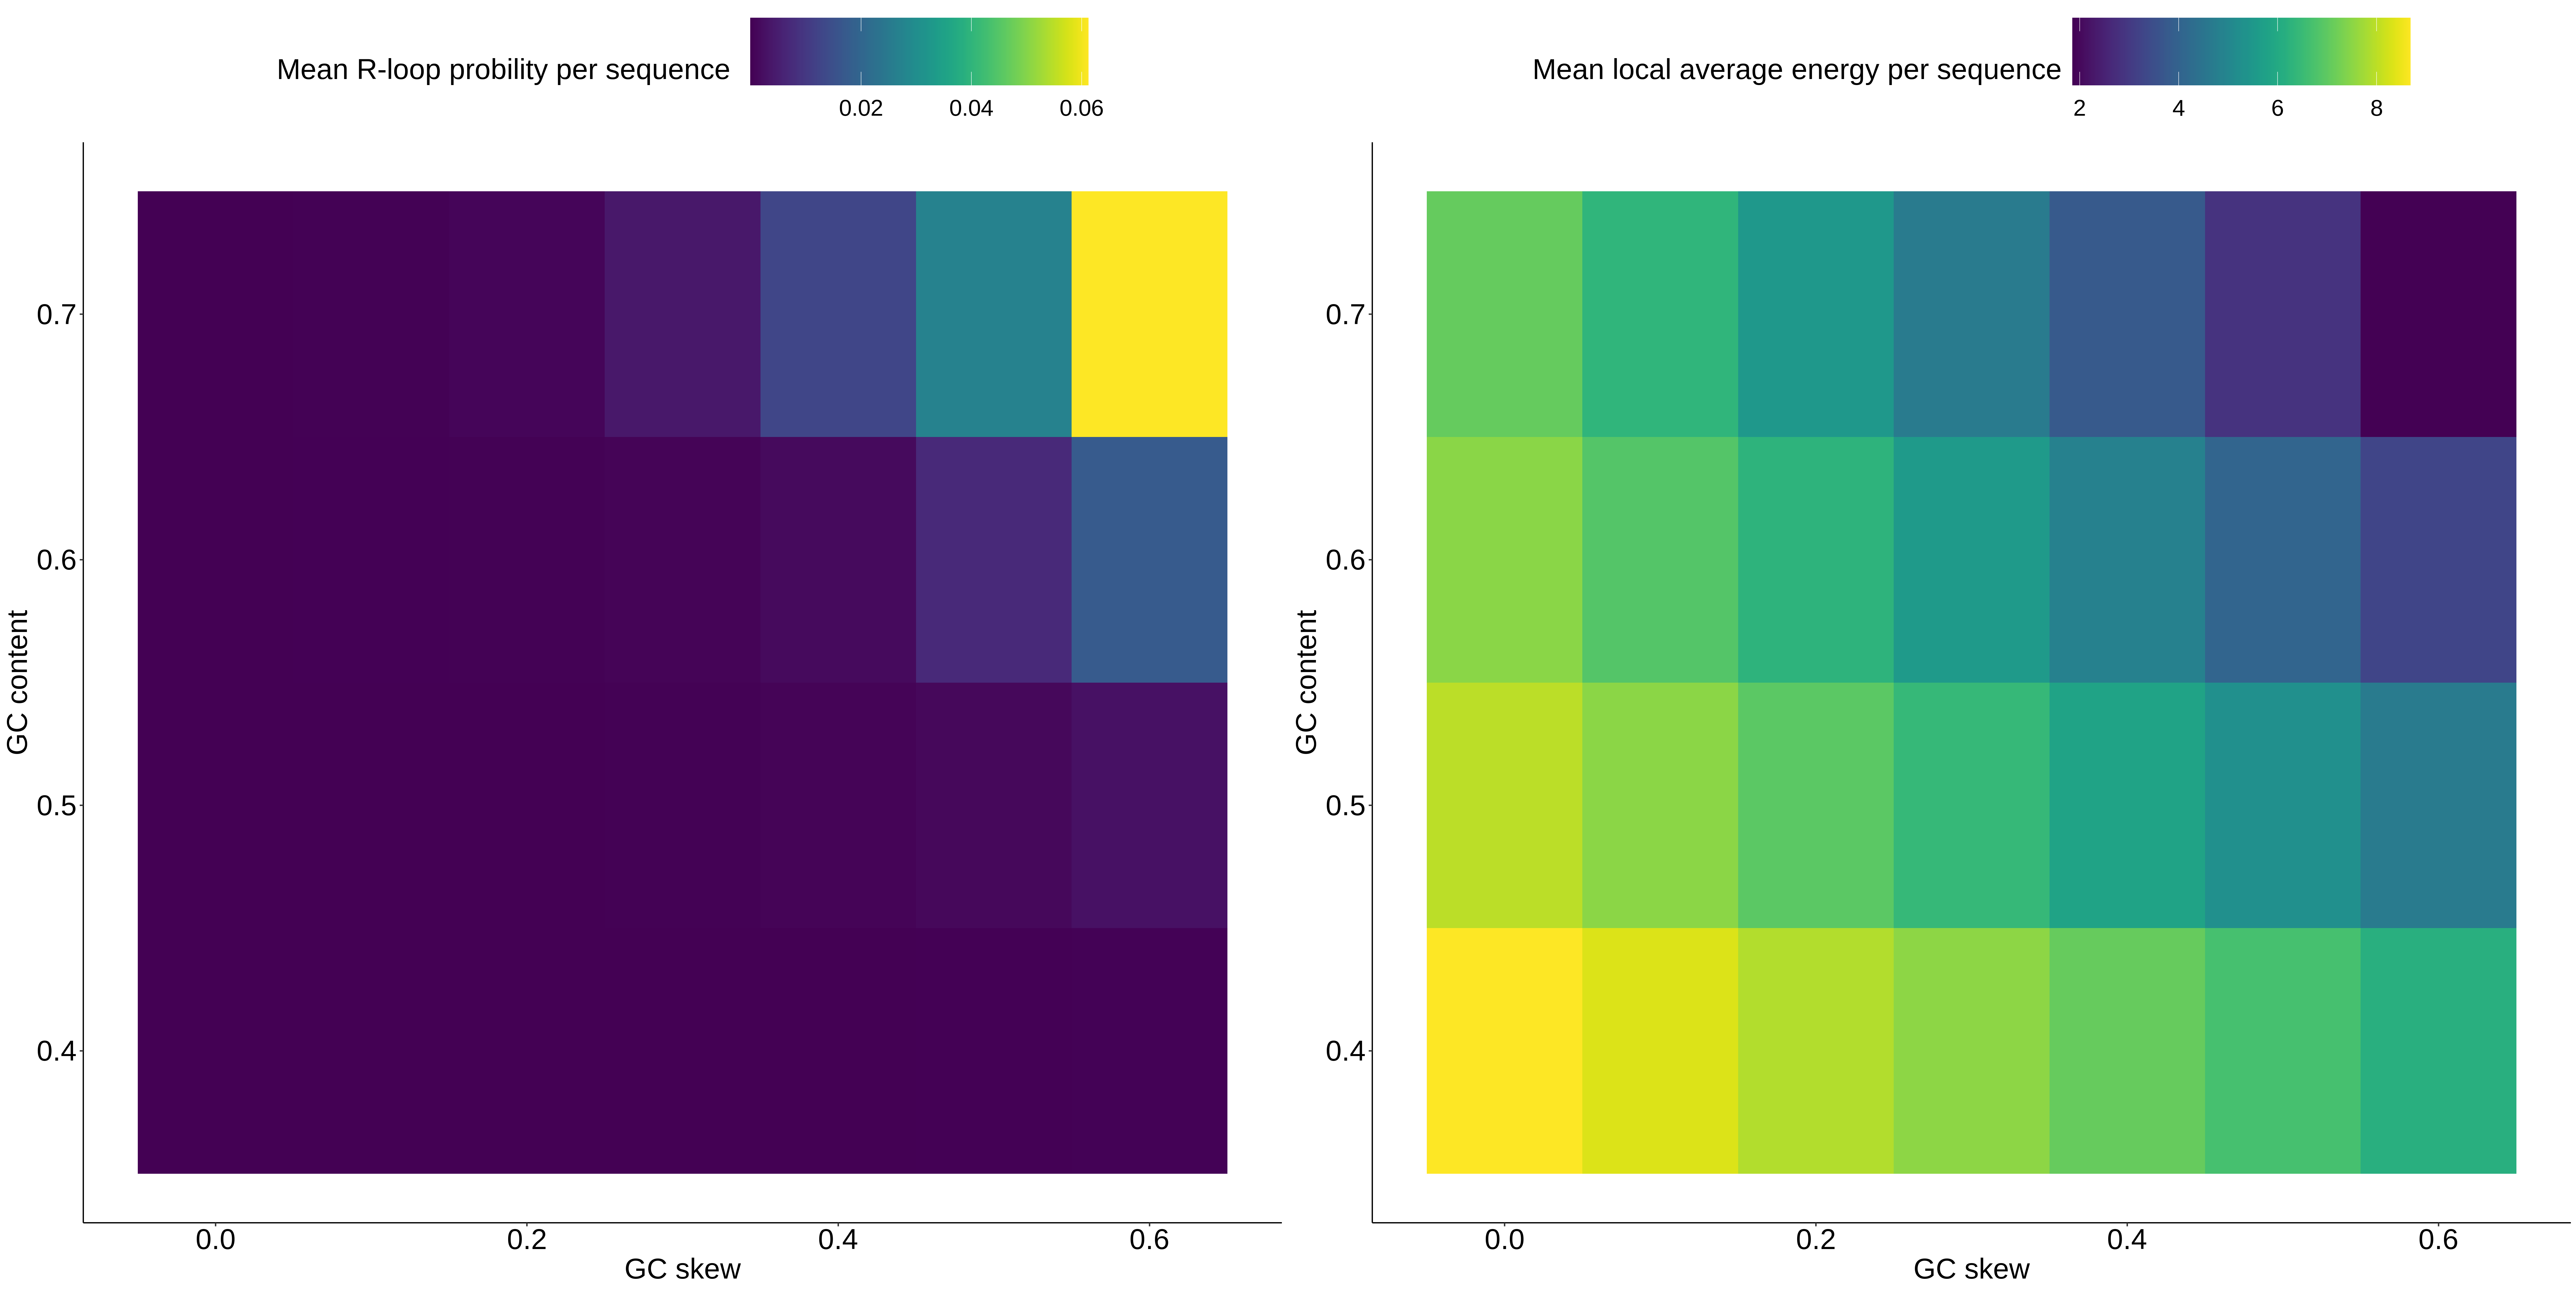
\includegraphics[width=14cm]{images/plots/rlooper_expect_tile.png}
	\centering
	\caption{Heatmaps showing mean R-loop probability per sequence (left) and mean local average energy per sequence (right) for 100 sequences of length 200 at various levels of GC skew and content. As GC skew and content increase, the mean R-loop probability also increases while the mean local average energy tends to decrease. This aligns with the basic expectation that increased GC skew and content favor R-loop formation.}
	\label{fig:rlooper-expect}
\end{figure}

Both local average energy and somewhat consequentially, mean R-loop probability are sensitive to both the GC skew and content of the input sequence (fig \ref{fig:rlooper-expect}). Comparing between sequences generated with the same parameters and therefore GC skew and content ensures that we are mainly evaluating how the arrangement of a particular set of nucleotides is predicted in generally effect the likelihood of R-loop formation.


\paragraph{RNA secondary structure}

Significant amounts of RNA secondary structure, especially large hairpins, are expected to reduce the likelihood of R-loop formation by causing competition for binding to the nascent RNA strand between itself and the DNA template. To avoid selecting sequences that are predicted to form an anomalous degree of RNA secondary structure SPOT-RNA rNA secondary structure prediction program in conjunction with the bpRNA structure annotation program \cite{Singh2019, Danaee2018} were used to calculate the estimated proportion of ribonucleotides in a given transcribed variable region that would participate in hairpin structures (PH) and the estimated proportion that would remain unpaired (PUP). Candidate variable regions with low PH and high PUP were preferred.


\begin{figure}[H]
	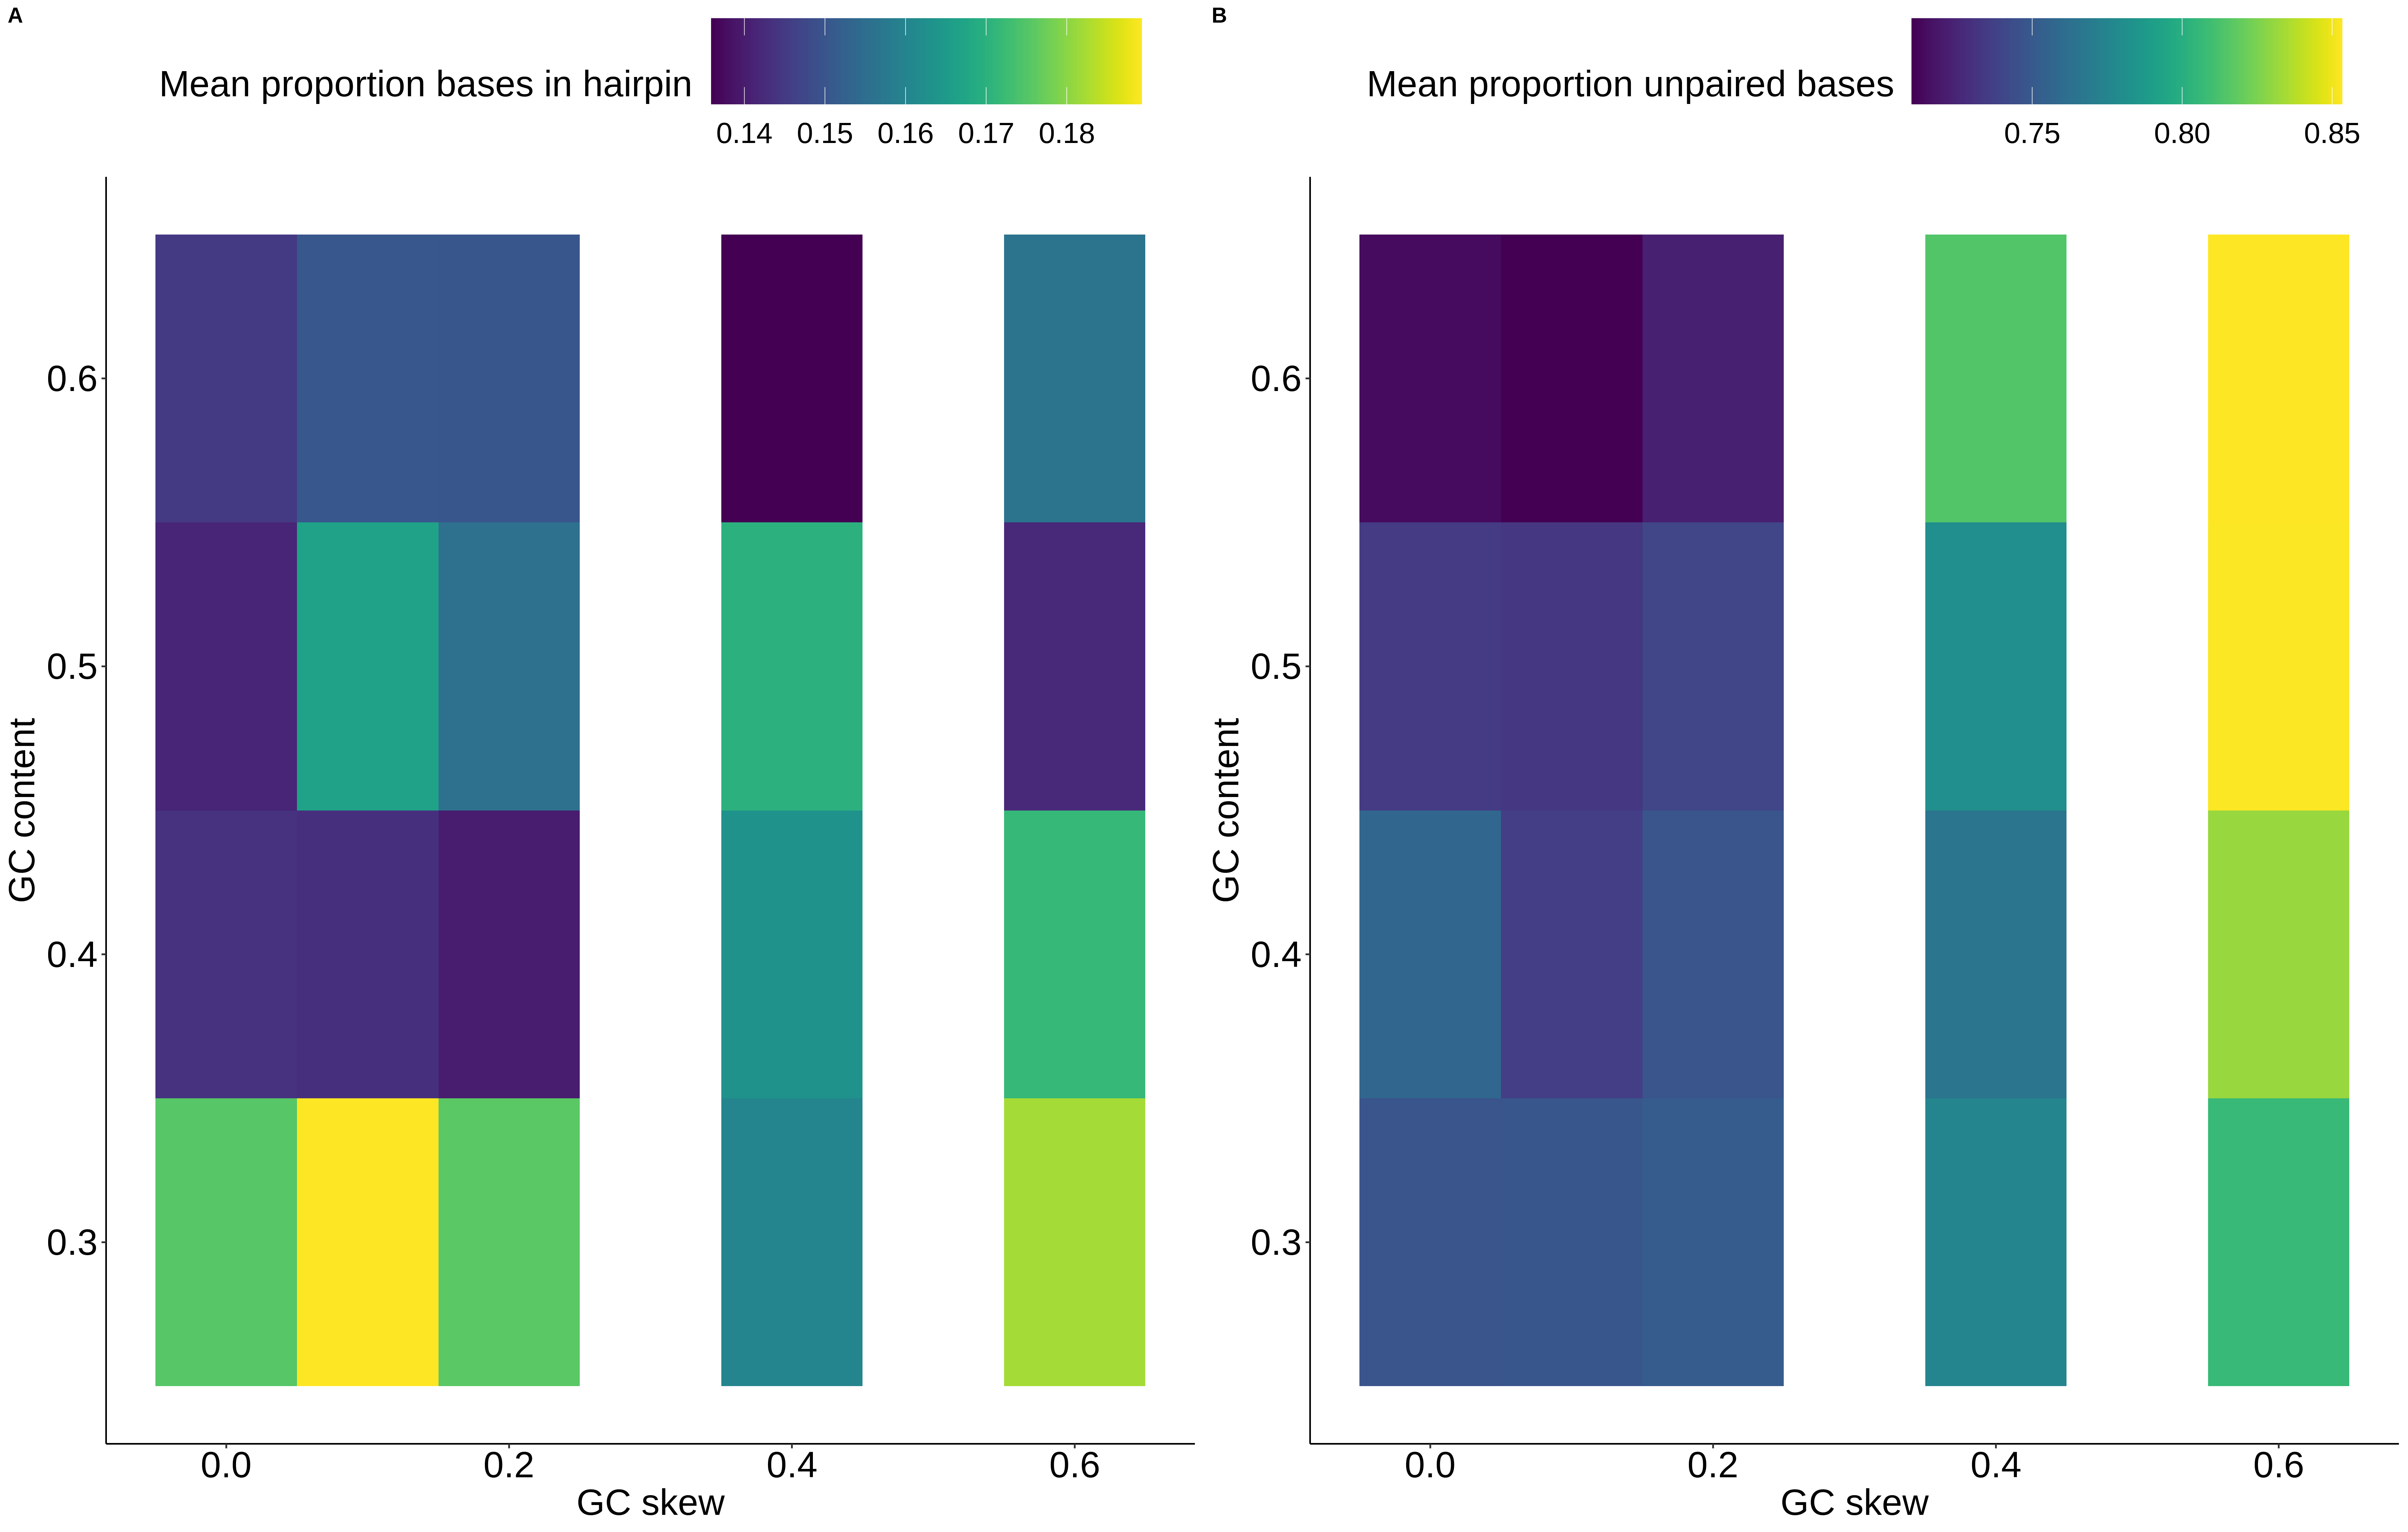
\includegraphics[width=14cm]{images/plots/rna_secondary_structure_temp.png}
	\centering
	\caption{Heatmaps showing PH (left) and PUP (right) for 100 candidate variable regions of length 200 at various levels of both GC skew and content.}
	\label{fig:rna_secondary_structure}
\end{figure}


\subsubsection{EcoRI site and 3' homology arm}

The final 30 nucleotides of each insert will be composed of a EcoRI recognition site (6 bp) and the 3' homology arm (24 bp). 

\begin{figure}[H]
	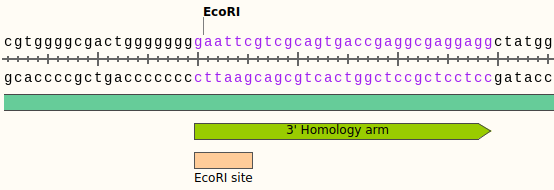
\includegraphics[width=10cm]{images/variable_region/3_homology_arm.png}
	\centering
	\caption{Sequence of the 3' homology arm and EcoRI site. The complete sequence is highlighted in purple.}
	\label{fig:3_prime_arm}
\end{figure}

Both the 5' homology arm + KpnI site and EcoRI site + 3' homology arm were produced using the Jupyter notebook available \href{https://github.com/EthanHolleman/plasmid-VR-design/blob/main/notes/homology_arms.ipynb}{at this link}.


\section{Assembly of DNA inserts}

Complete insert sequences will be cloned into three different plasmid backbones: pFC9 (fig \ref{fig:map_pFC8}), pFC8 (fig \ref{fig:map_pFC8}), and pFC53tacT$_1$T$_2$ (fig \ref{fig:map_pFC53tacT1T2}). pFC9 will be utilized for testing R-loop initiation, pFC8 for R-loop termination and pFC53tacT$_1$T$_2$ for multiple and single-round transcription versions of both initiation and termination experiments with Tac polymerase. 


\begin{figure}[H]
	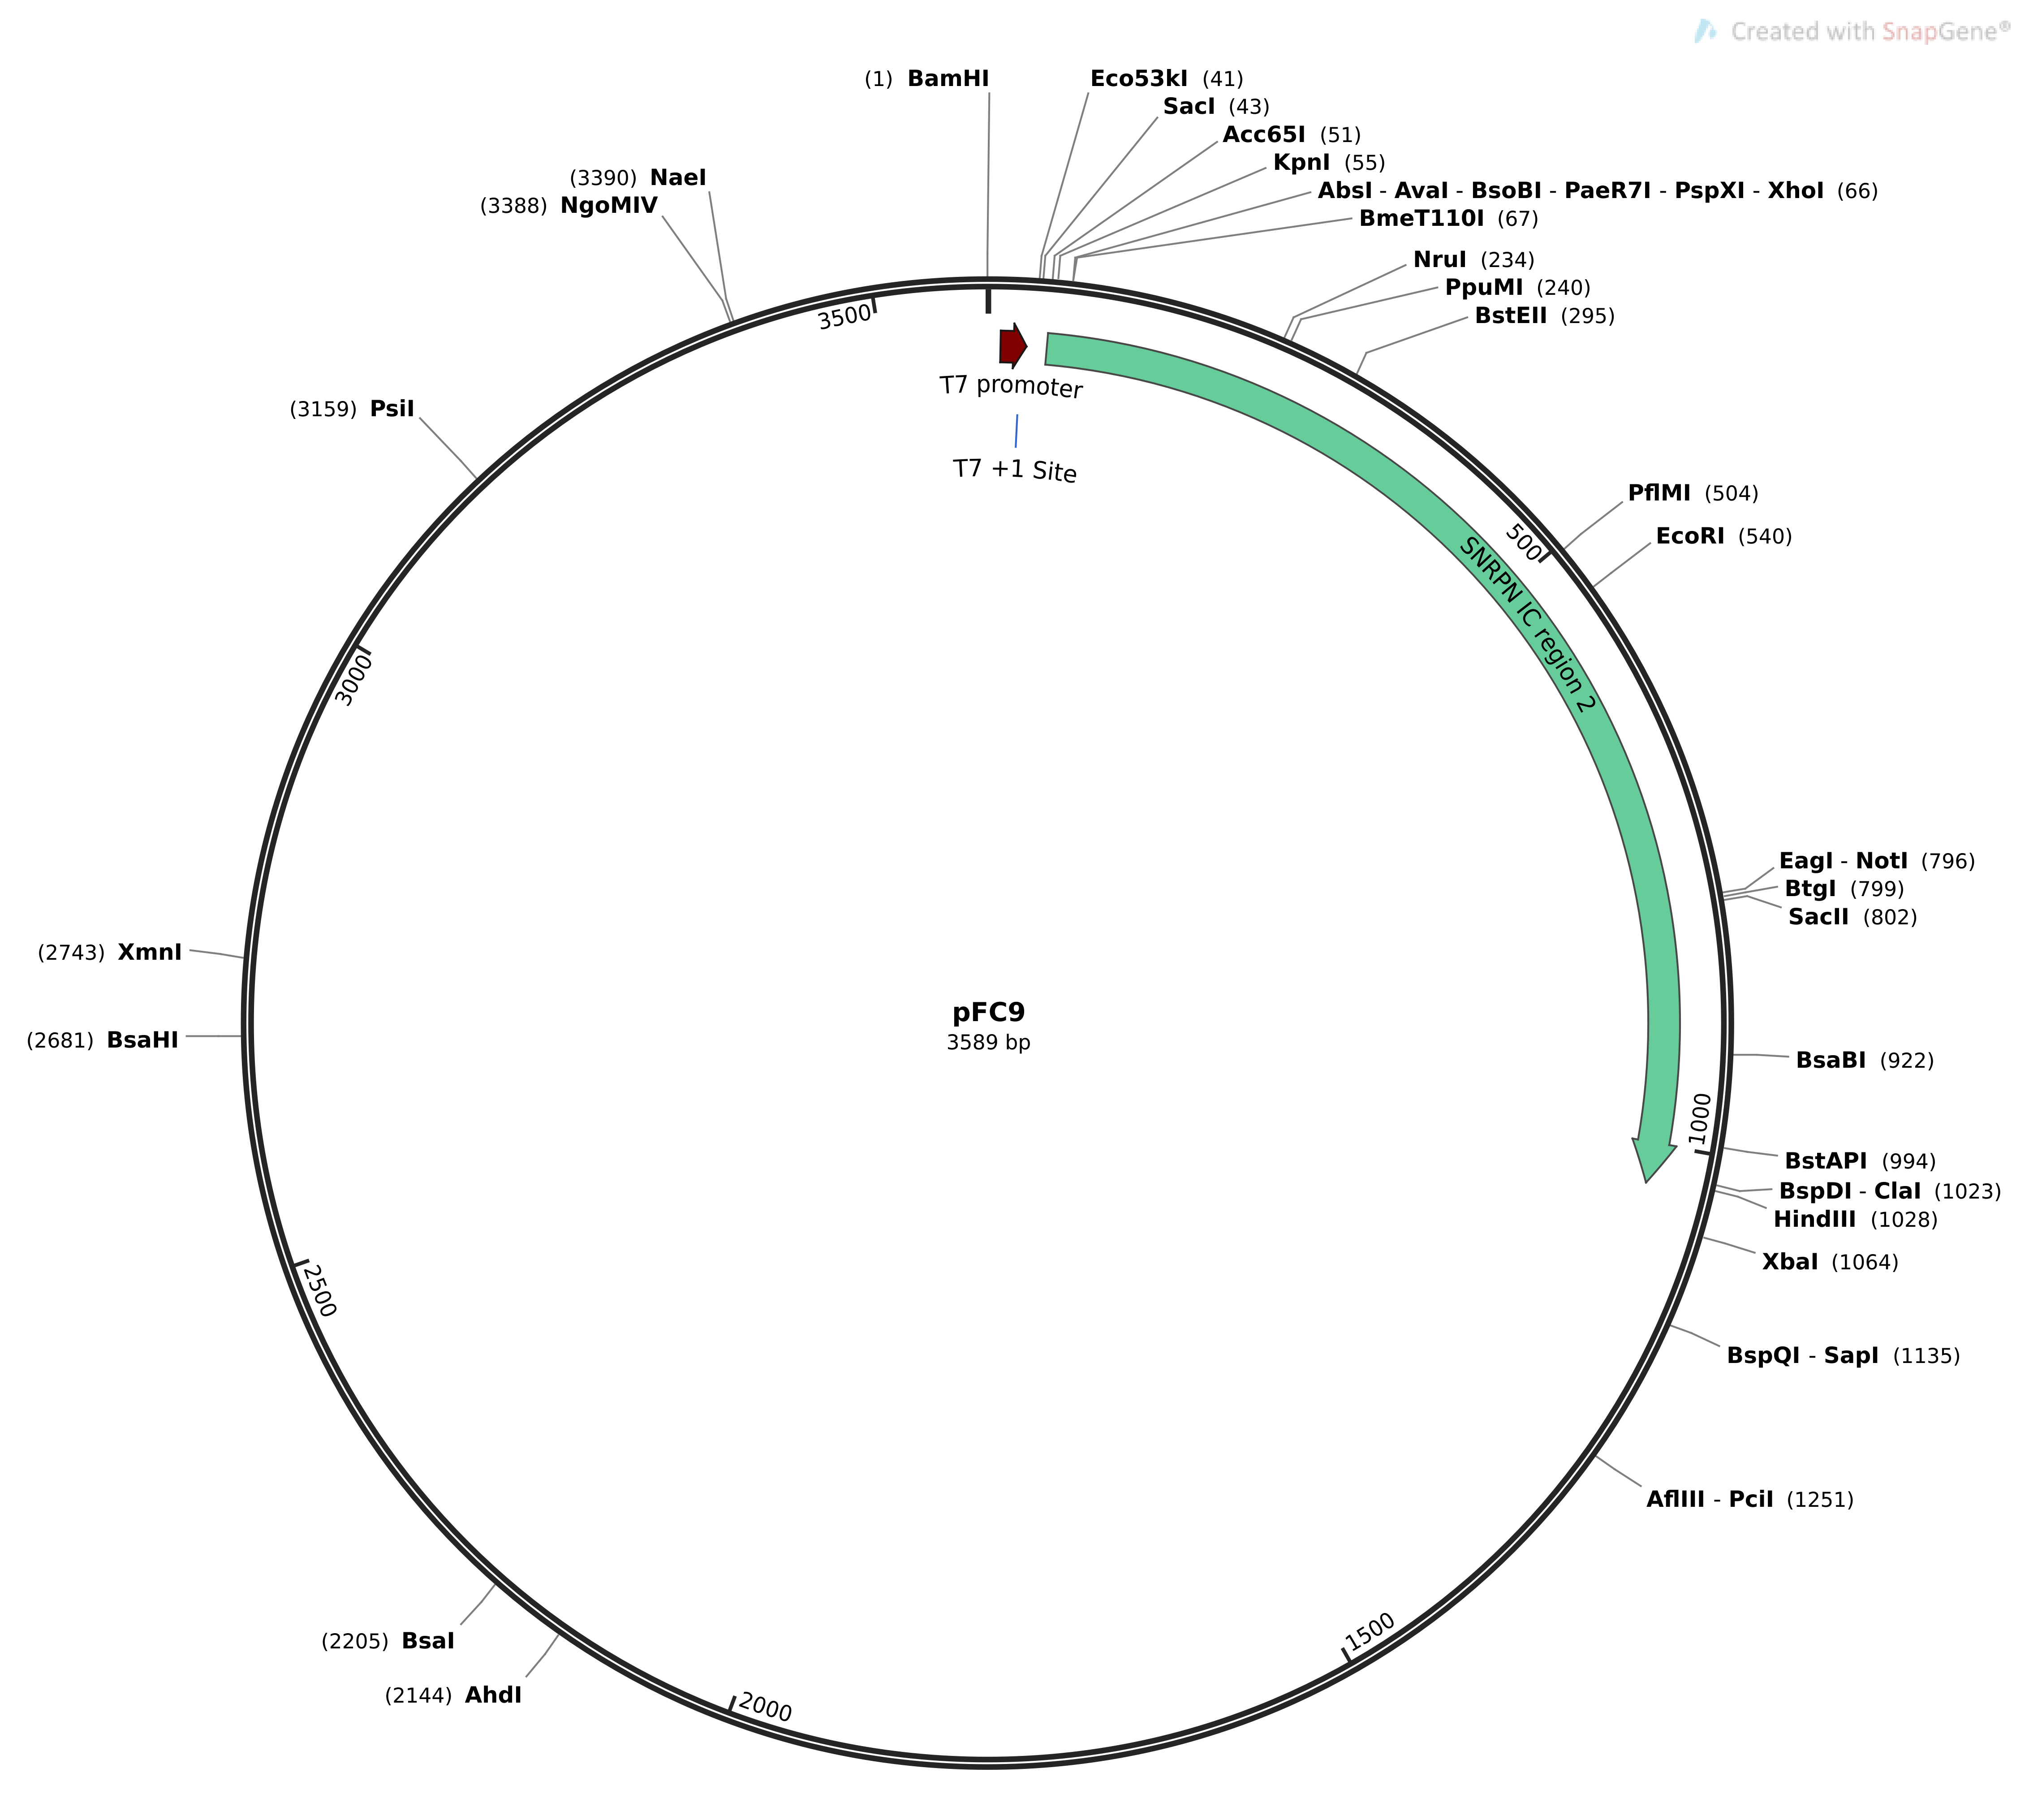
\includegraphics[width=8cm]{images/plasmid_maps/pFC9_Map.png}
	\centering
	\caption{Map of pFC9.}
	\label{fig:map_pFC9}
\end{figure}


\begin{figure}[H]
	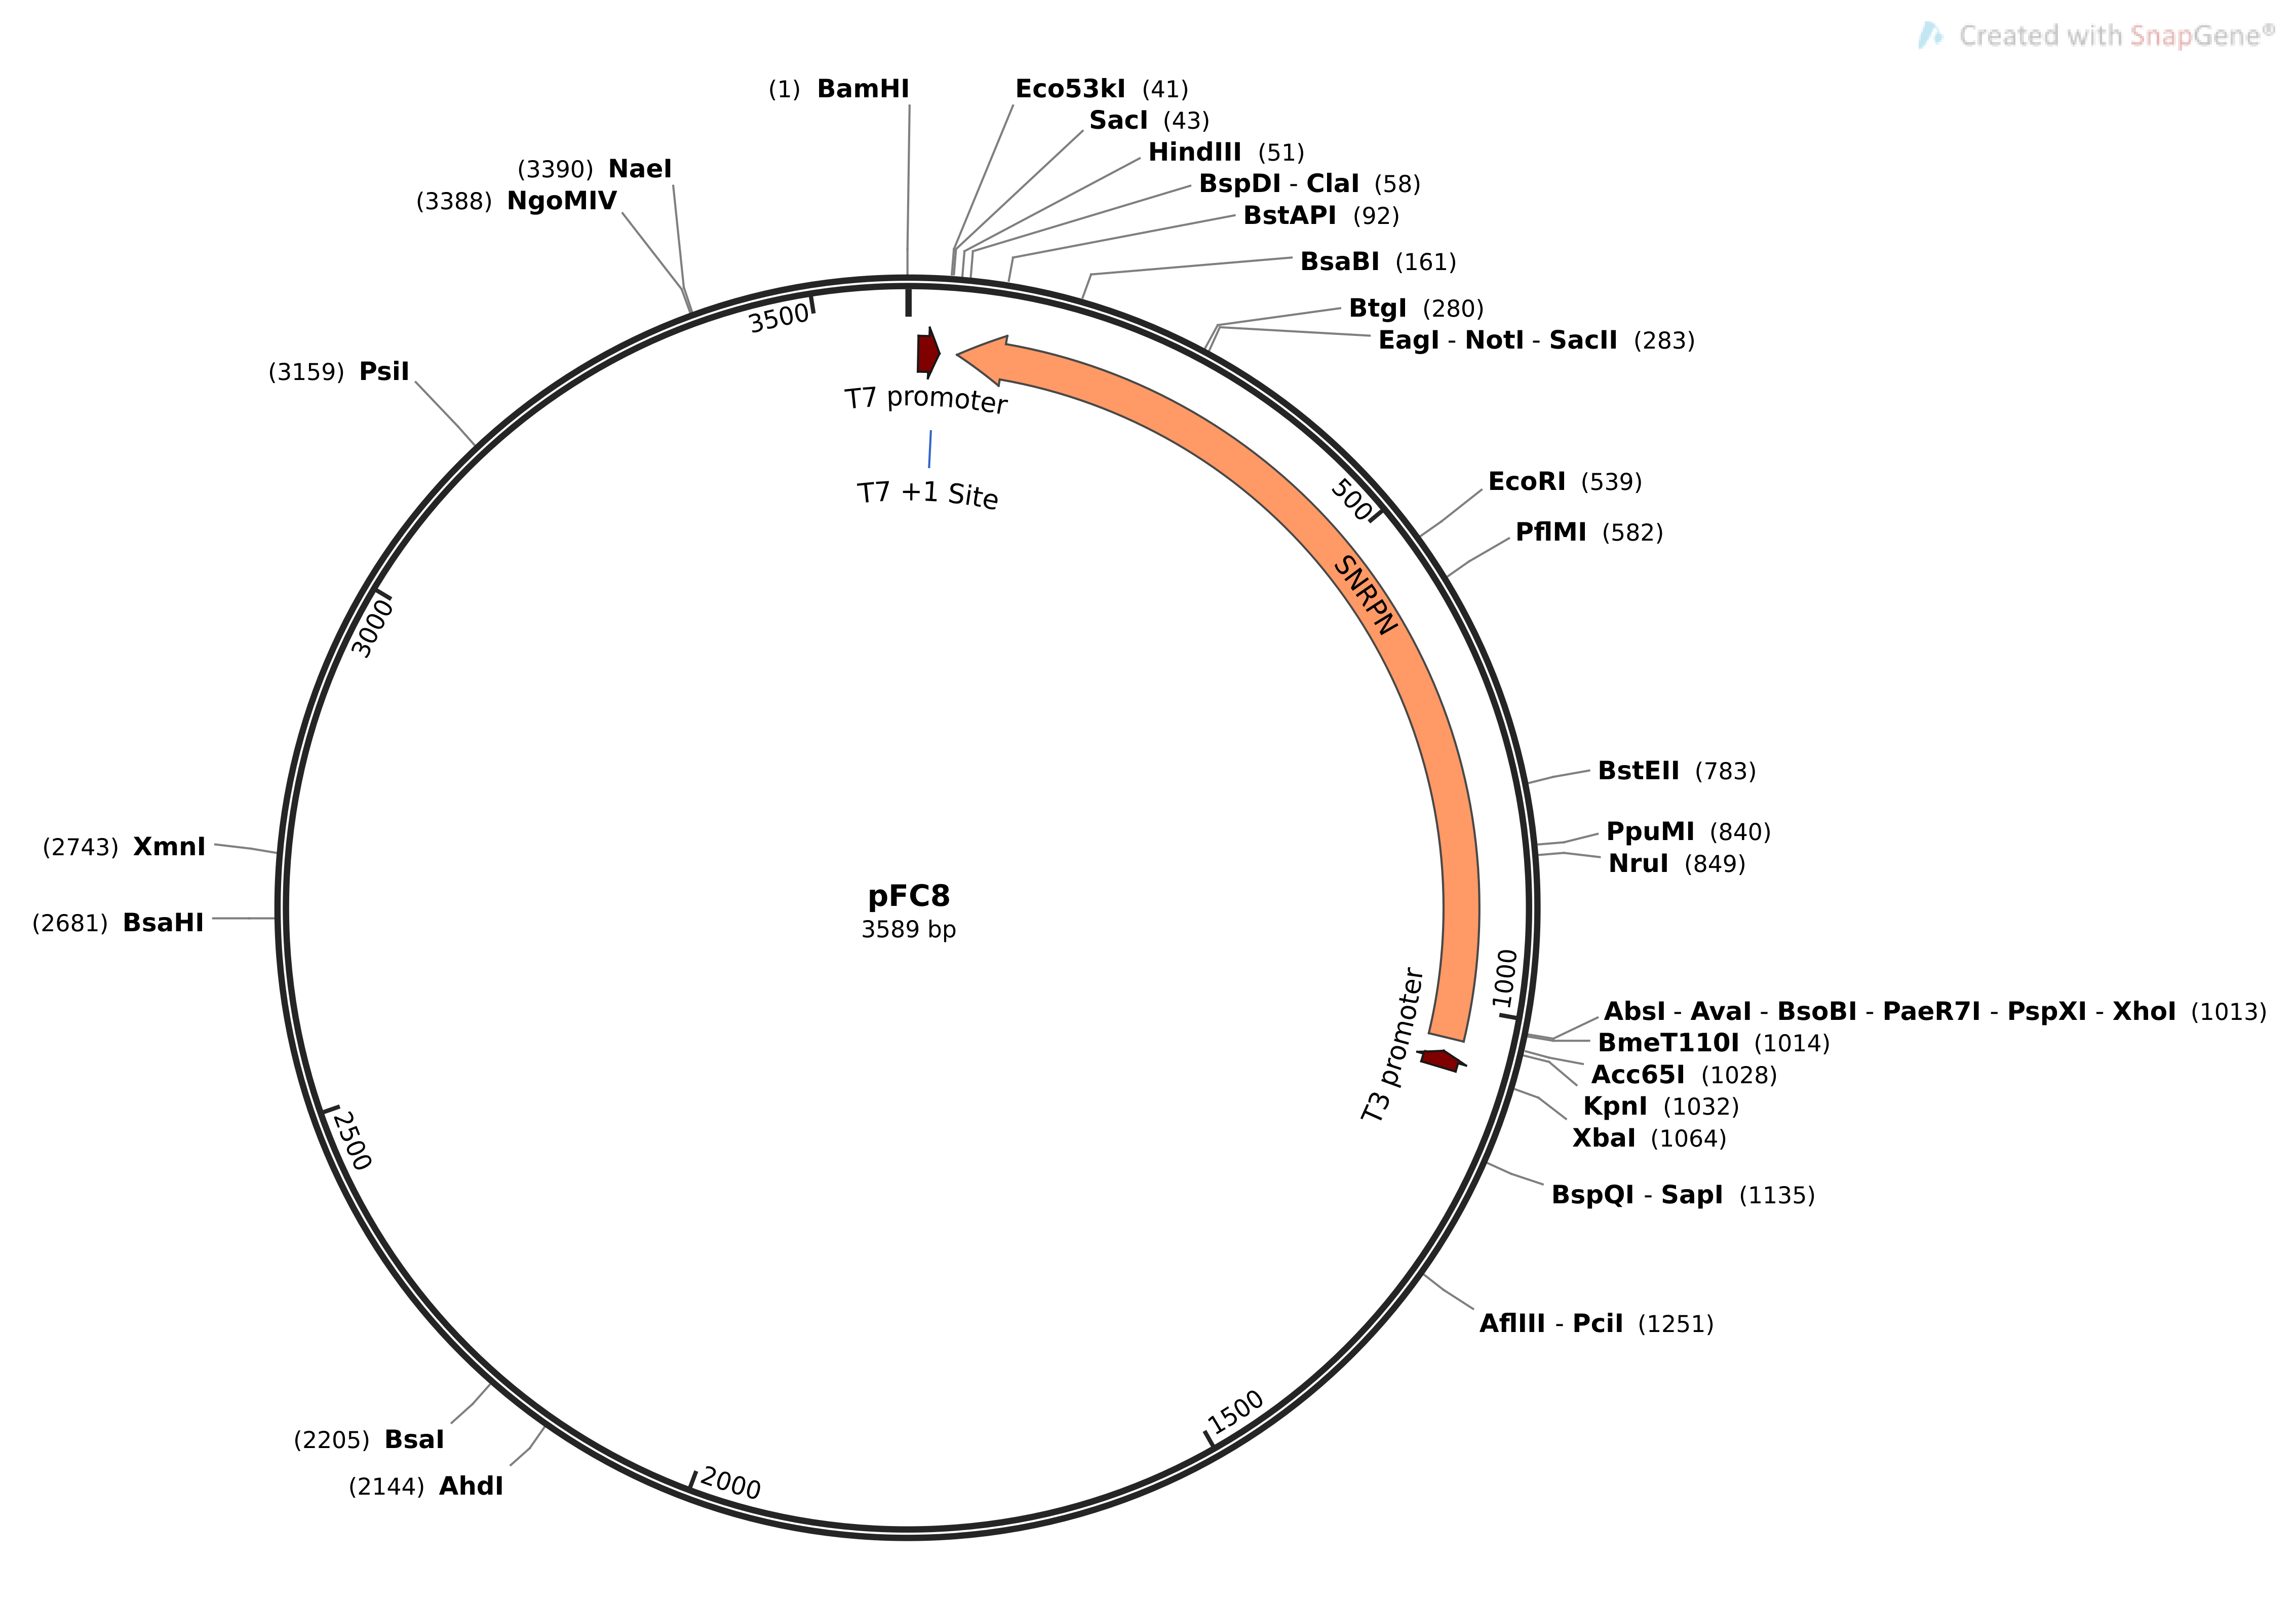
\includegraphics[width=11cm]{images/plasmid_maps/pFC8_Map.png}
	\centering
	\caption{Map of pFC8.}
	\label{fig:map_pFC8}
\end{figure}


\begin{figure}[H]
	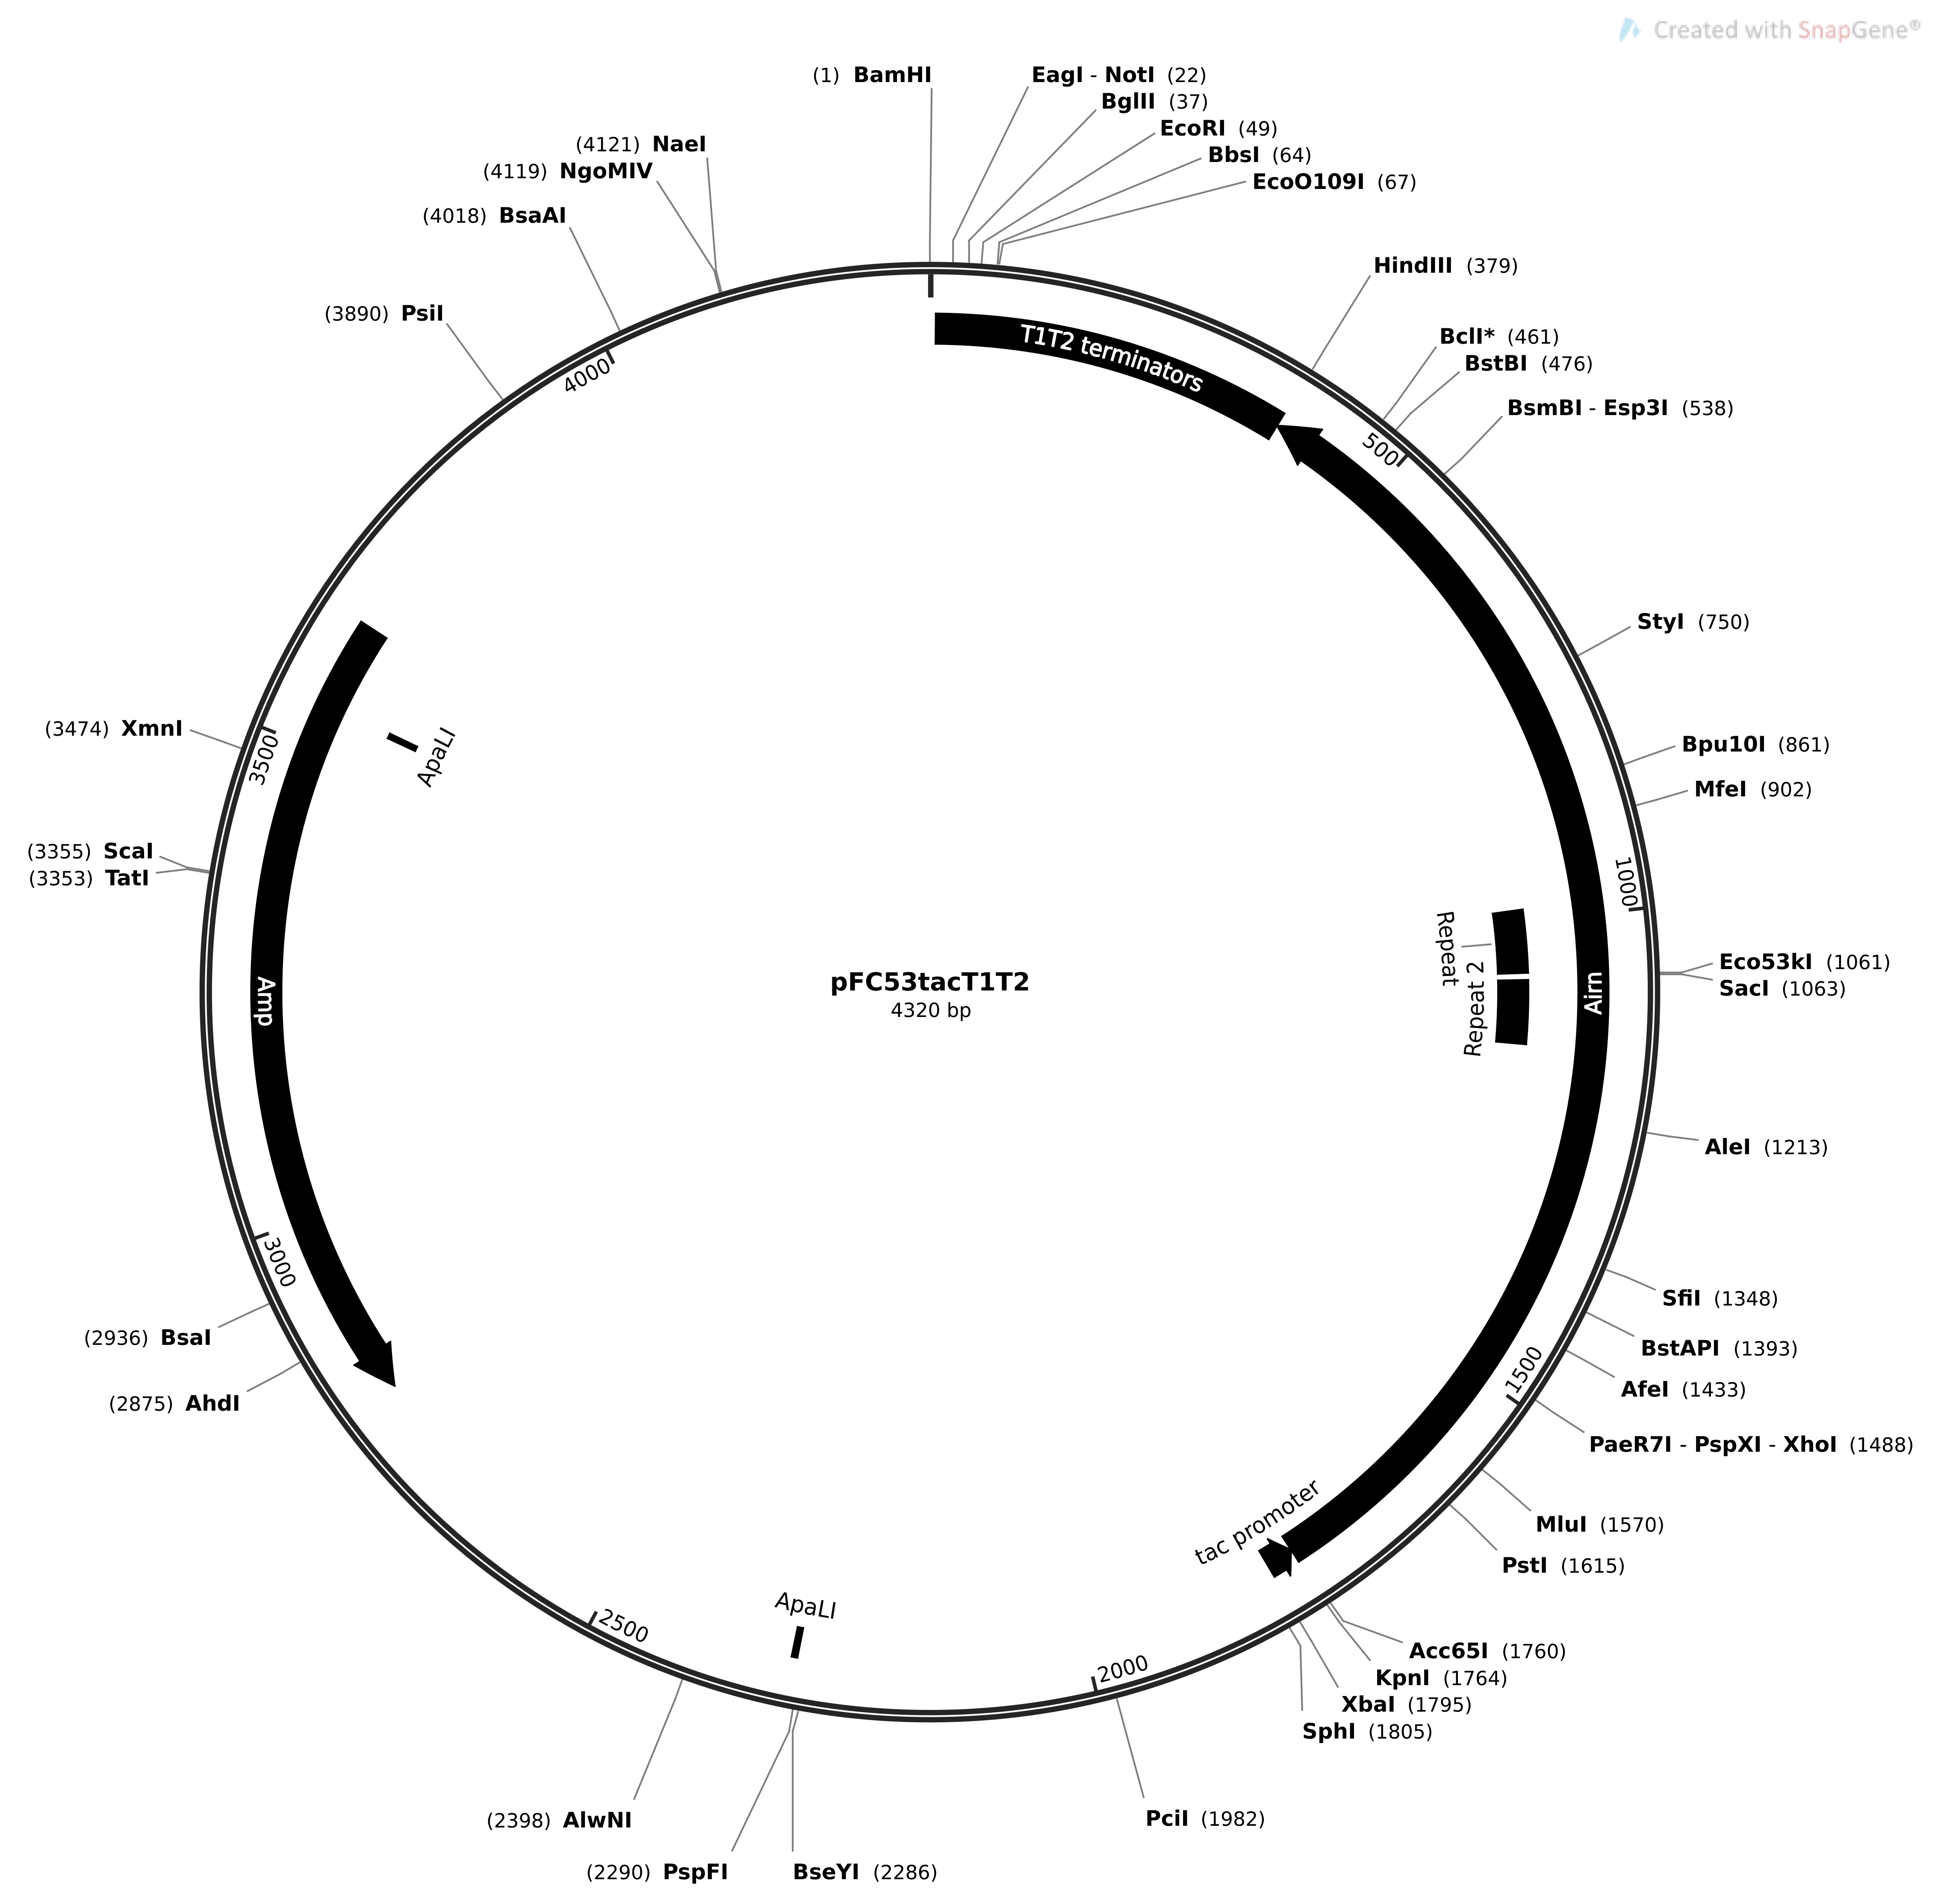
\includegraphics[width=8cm]{images/plasmid_maps/pFC53tacT1T2_Map.png}
	\centering
	\caption{Map of pFC53tacT$_1$T$_2$.}
	\label{fig:map_pFC53tacT1T2}
\end{figure}


\subsection{T7 initiation series constructs}
\label{T7:init} 


\begin{figure}[H]
	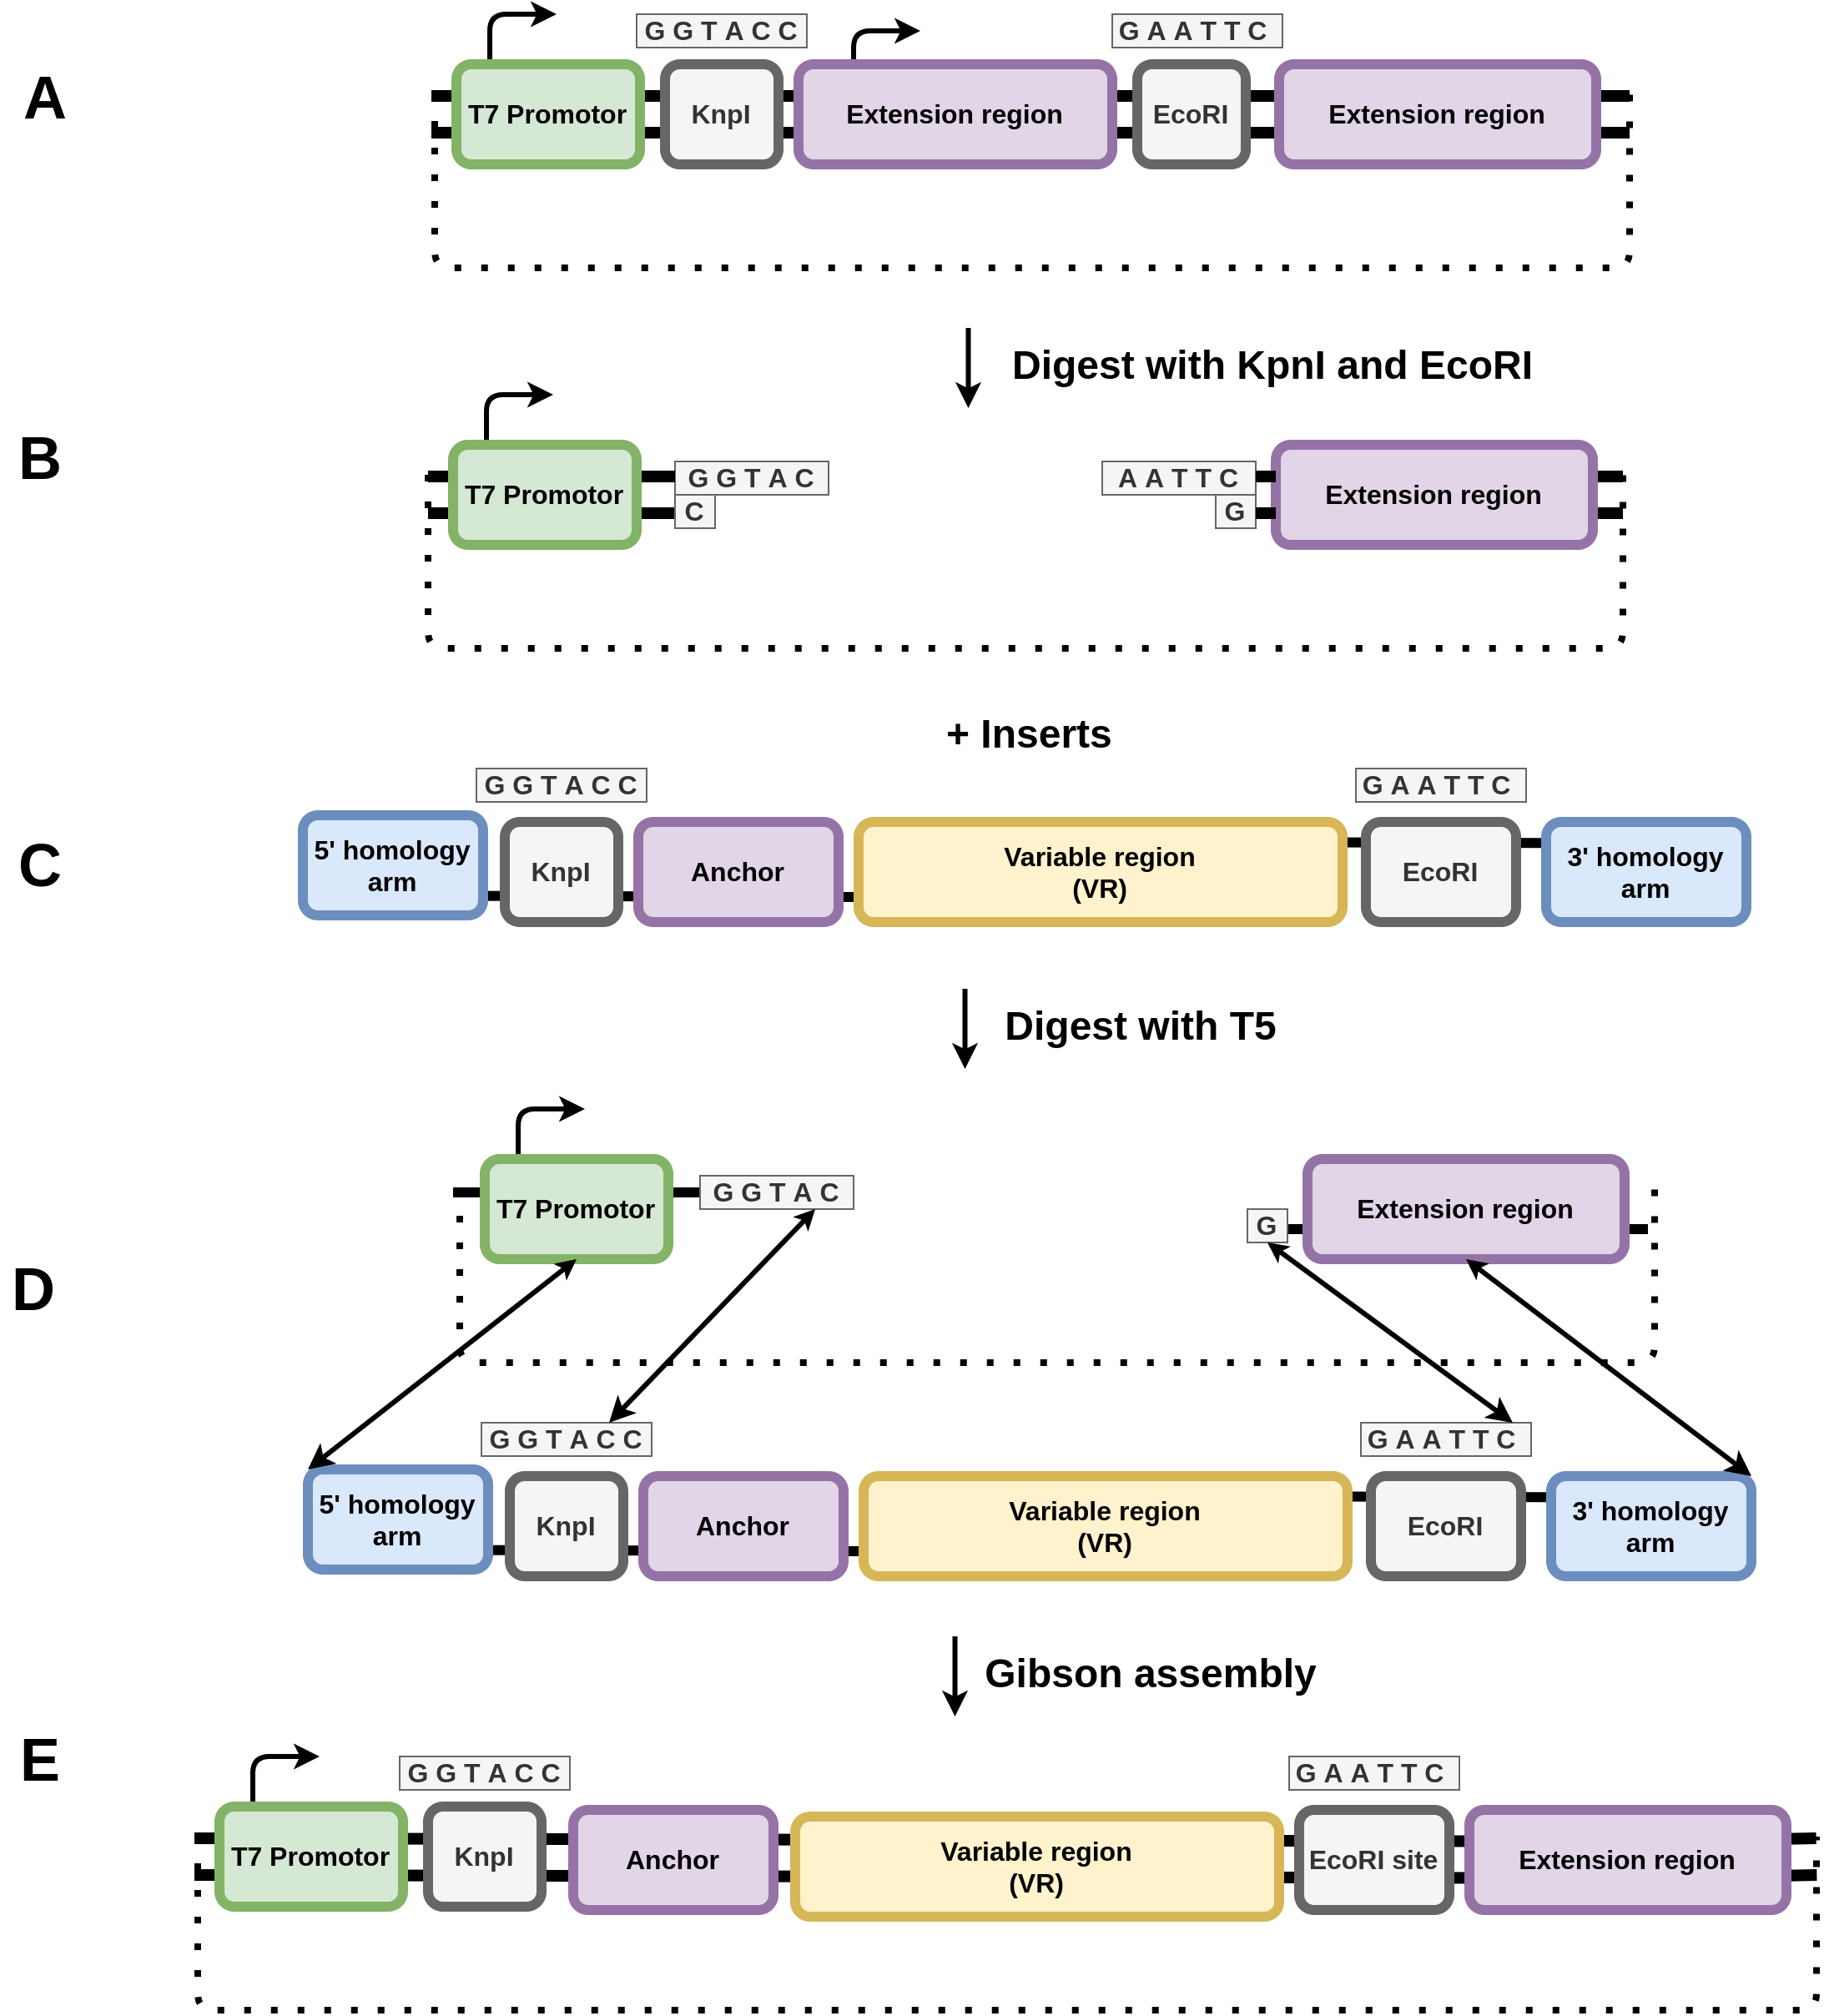
\includegraphics[width=15cm]{images/cloning_diagrams/construct_diagrams-T7-Initiation-series.png}
	\centering
	\caption{Diagram of pFC9 T7 insertion series cloning strategy.}
	\label{clone:T7-insert}
\end{figure}

First, pFC9 will be linearized by digestion with KpnI and EcoRI  (fig \ref{clone:T7-insert}A). The large pFC9 fragment will then be purified via agarose gel and added to a mixture containing all insert sequences in equal molar concentrations (fig \ref{clone:T7-insert}B). Next, T5 exonuclease is added to digest the 5' ends of all DNA in the mixture. This will leave the 3' overhang of the digested KpnI site intact but degrade the 5' overhang of EcoRI  (fig \ref{clone:T7-insert}C). The 5' ends of the insert will also be degraded, exposing the complete KnpI and EcoRI sites. Next, during Gibson assembly the 5' homology arm and KnpI site will anneal to the pFC9 large fragment, overhanging the digested KnpI site by 1 nucleotide. Similarly, the 3' homology arm and intact EcoRI site of the inserts will anneal to the pFC9 large fragment, with only the last nucleotide (C) of the insert's intact EcoRI site annealing to the 3' G present at the digested EcoRI site of the pFC9 large fragment (fig \ref{clone:T7-insert}D). This will result in a library of circular constructs with all inserts located downstream of and oriented forward relative to, the pFC9 T7 promoter (fig \ref{clone:T7-insert}). 

\begin{figure}[H]
	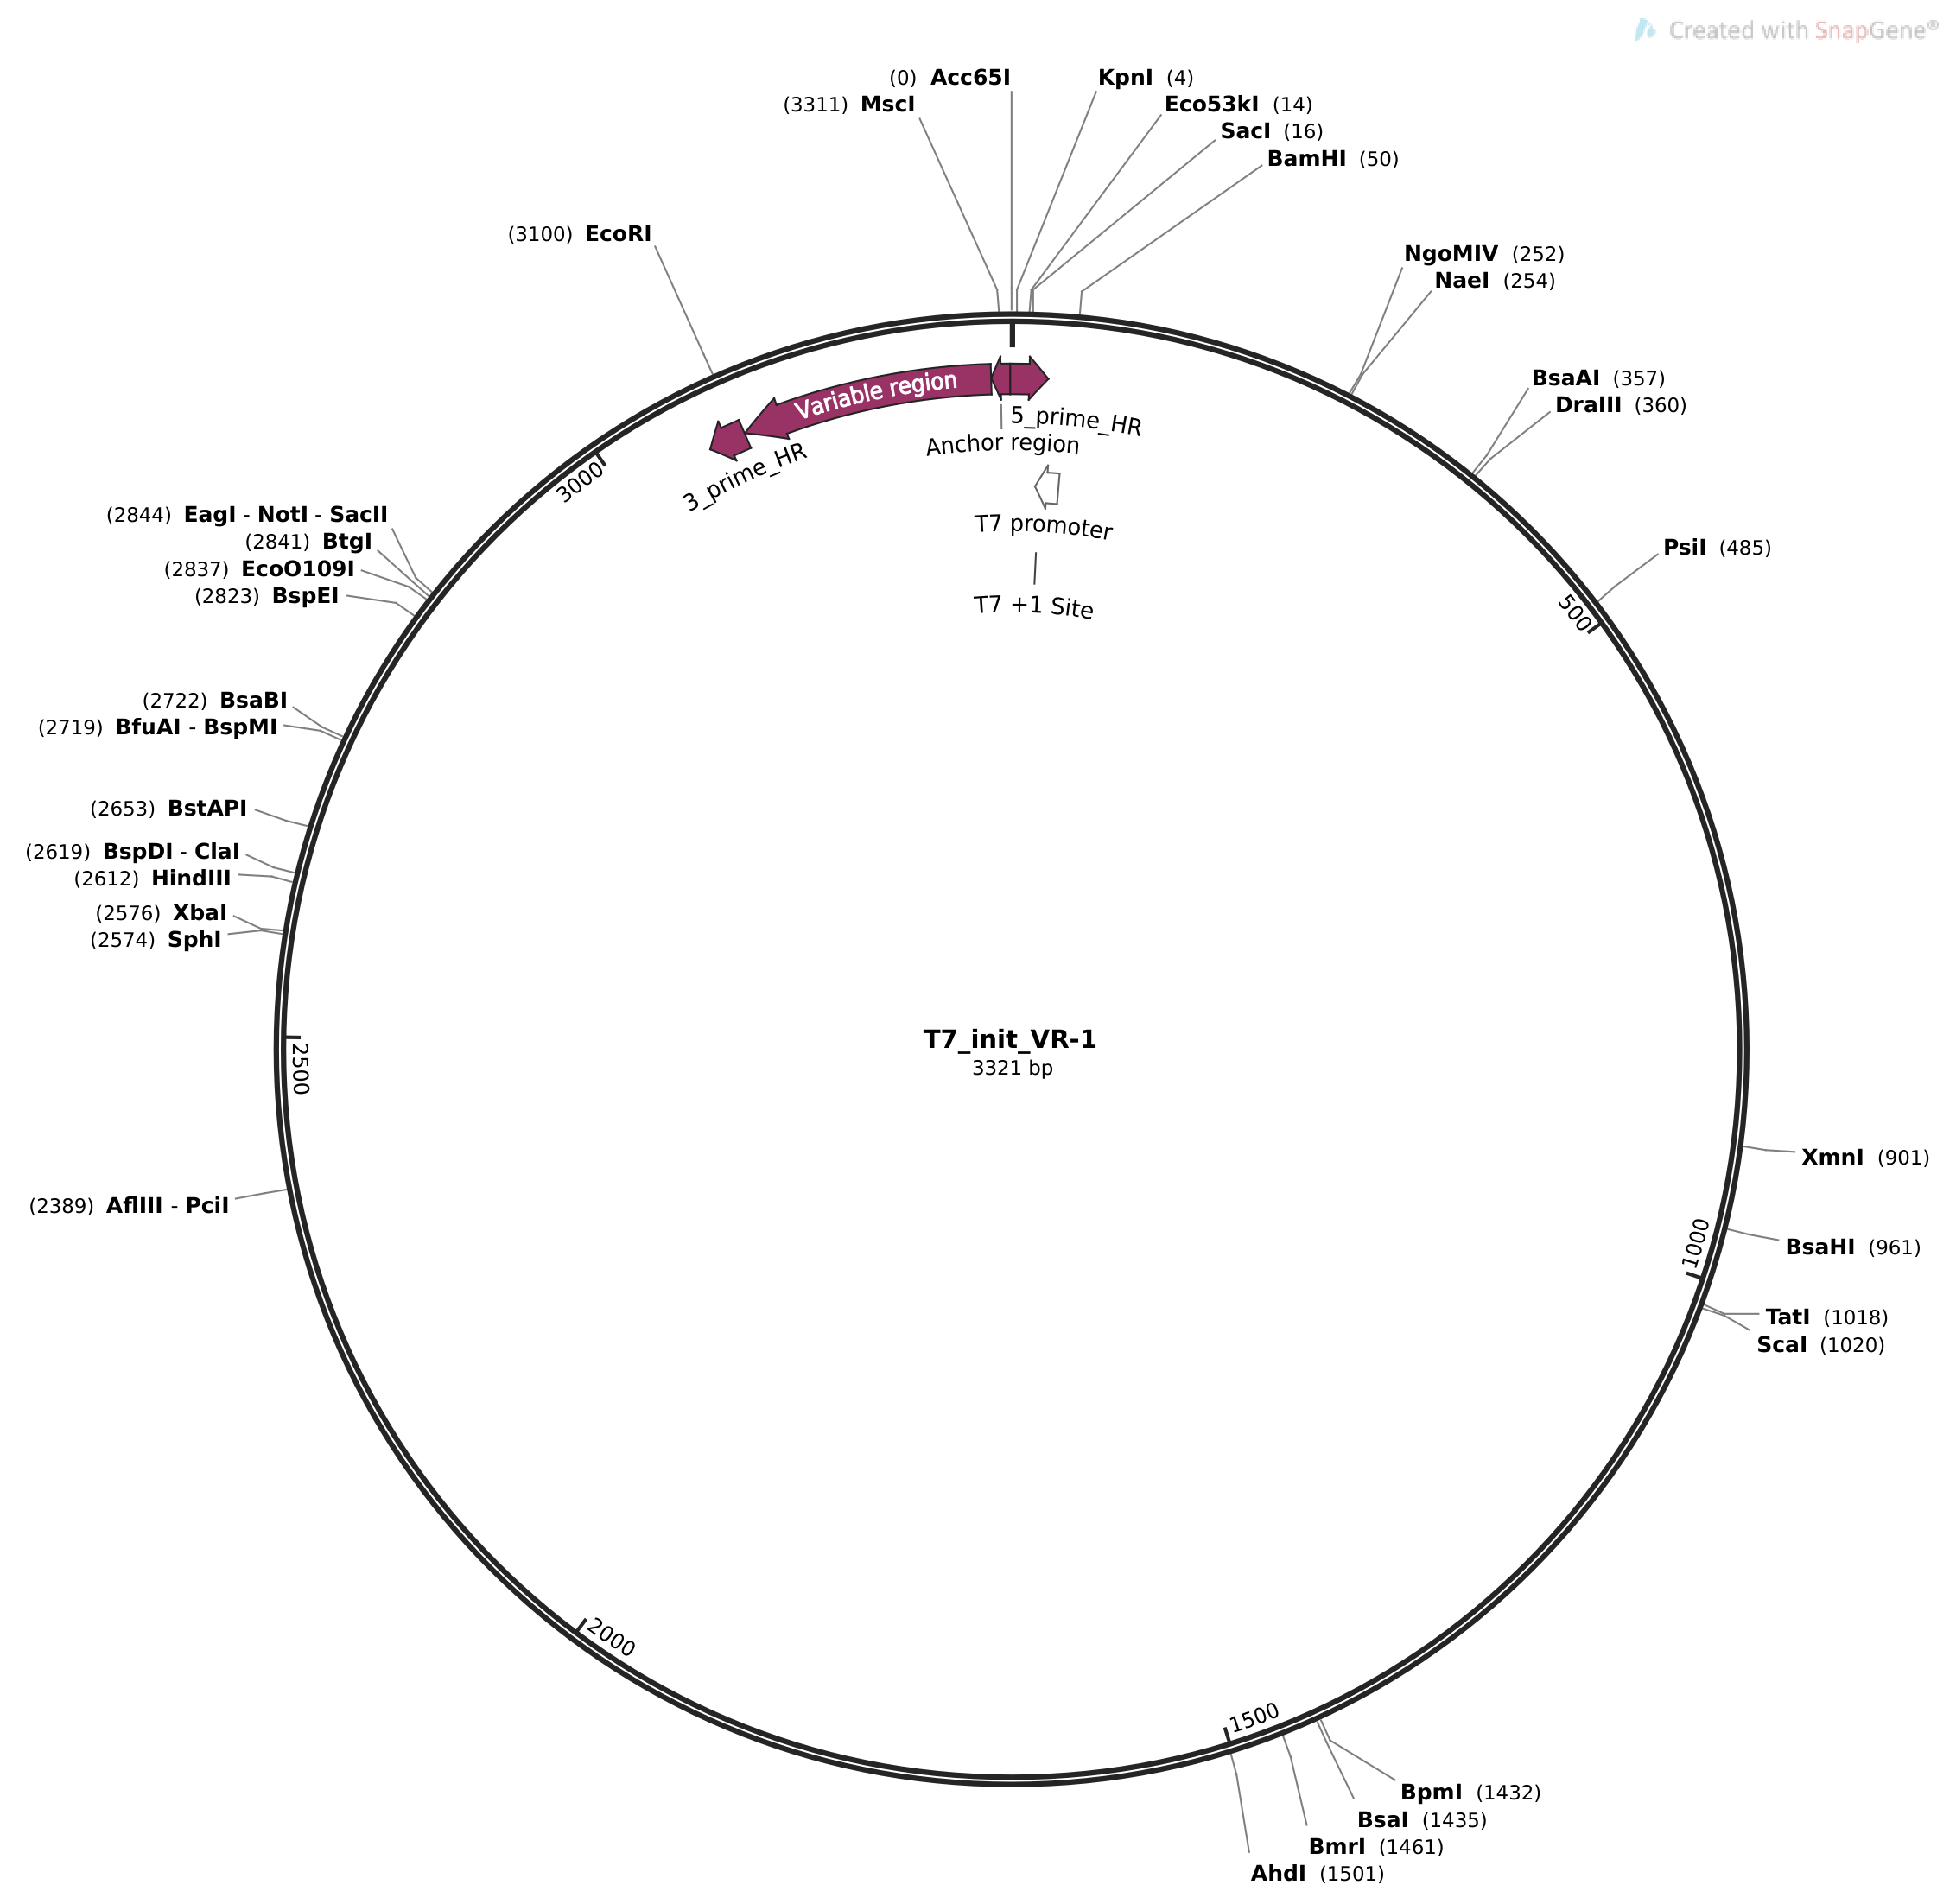
\includegraphics[width=12cm]{images/plasmid_maps/T7_init_vr-1_simulated_assembly.png}
	\centering
	\caption{Plasmid map of produced by simulating the T7 initiation series cloning protocol for the insert containing variable region 1. Cloning simulations were ran and confirmed to be successful for all complete inserts sequences.}
	\label{clone:T7-insert-simulated}
\end{figure}

\subsubsection{Assembly protocol}

A Jupyter notebook for calculating the volumes of individual inserts, digested pFC9 backbone and Gibson assembly master mix to complete the Gibson assembly protocol outlined in fig \ref{clone:T7-insert-simulated} is available at this link. At the time of writing the concentration of pFC9 fragment and the concentrations of individual inserts are unknown and placeholder values that must be updated are currently used. All volumes and concentrations of reagents are derived from \href{https://www.neb.com/protocols/2012/12/11/gibson-assembly-protocol-e5510}{New England Biolabs Gibson assembly recommendations}.


\subsection{T7 termination series constructs}

After the successful sequencing of the T7 initiation series, pFC8 will be utilized as the backbone for construction of the termination series library. 

\begin{figure}[H]
	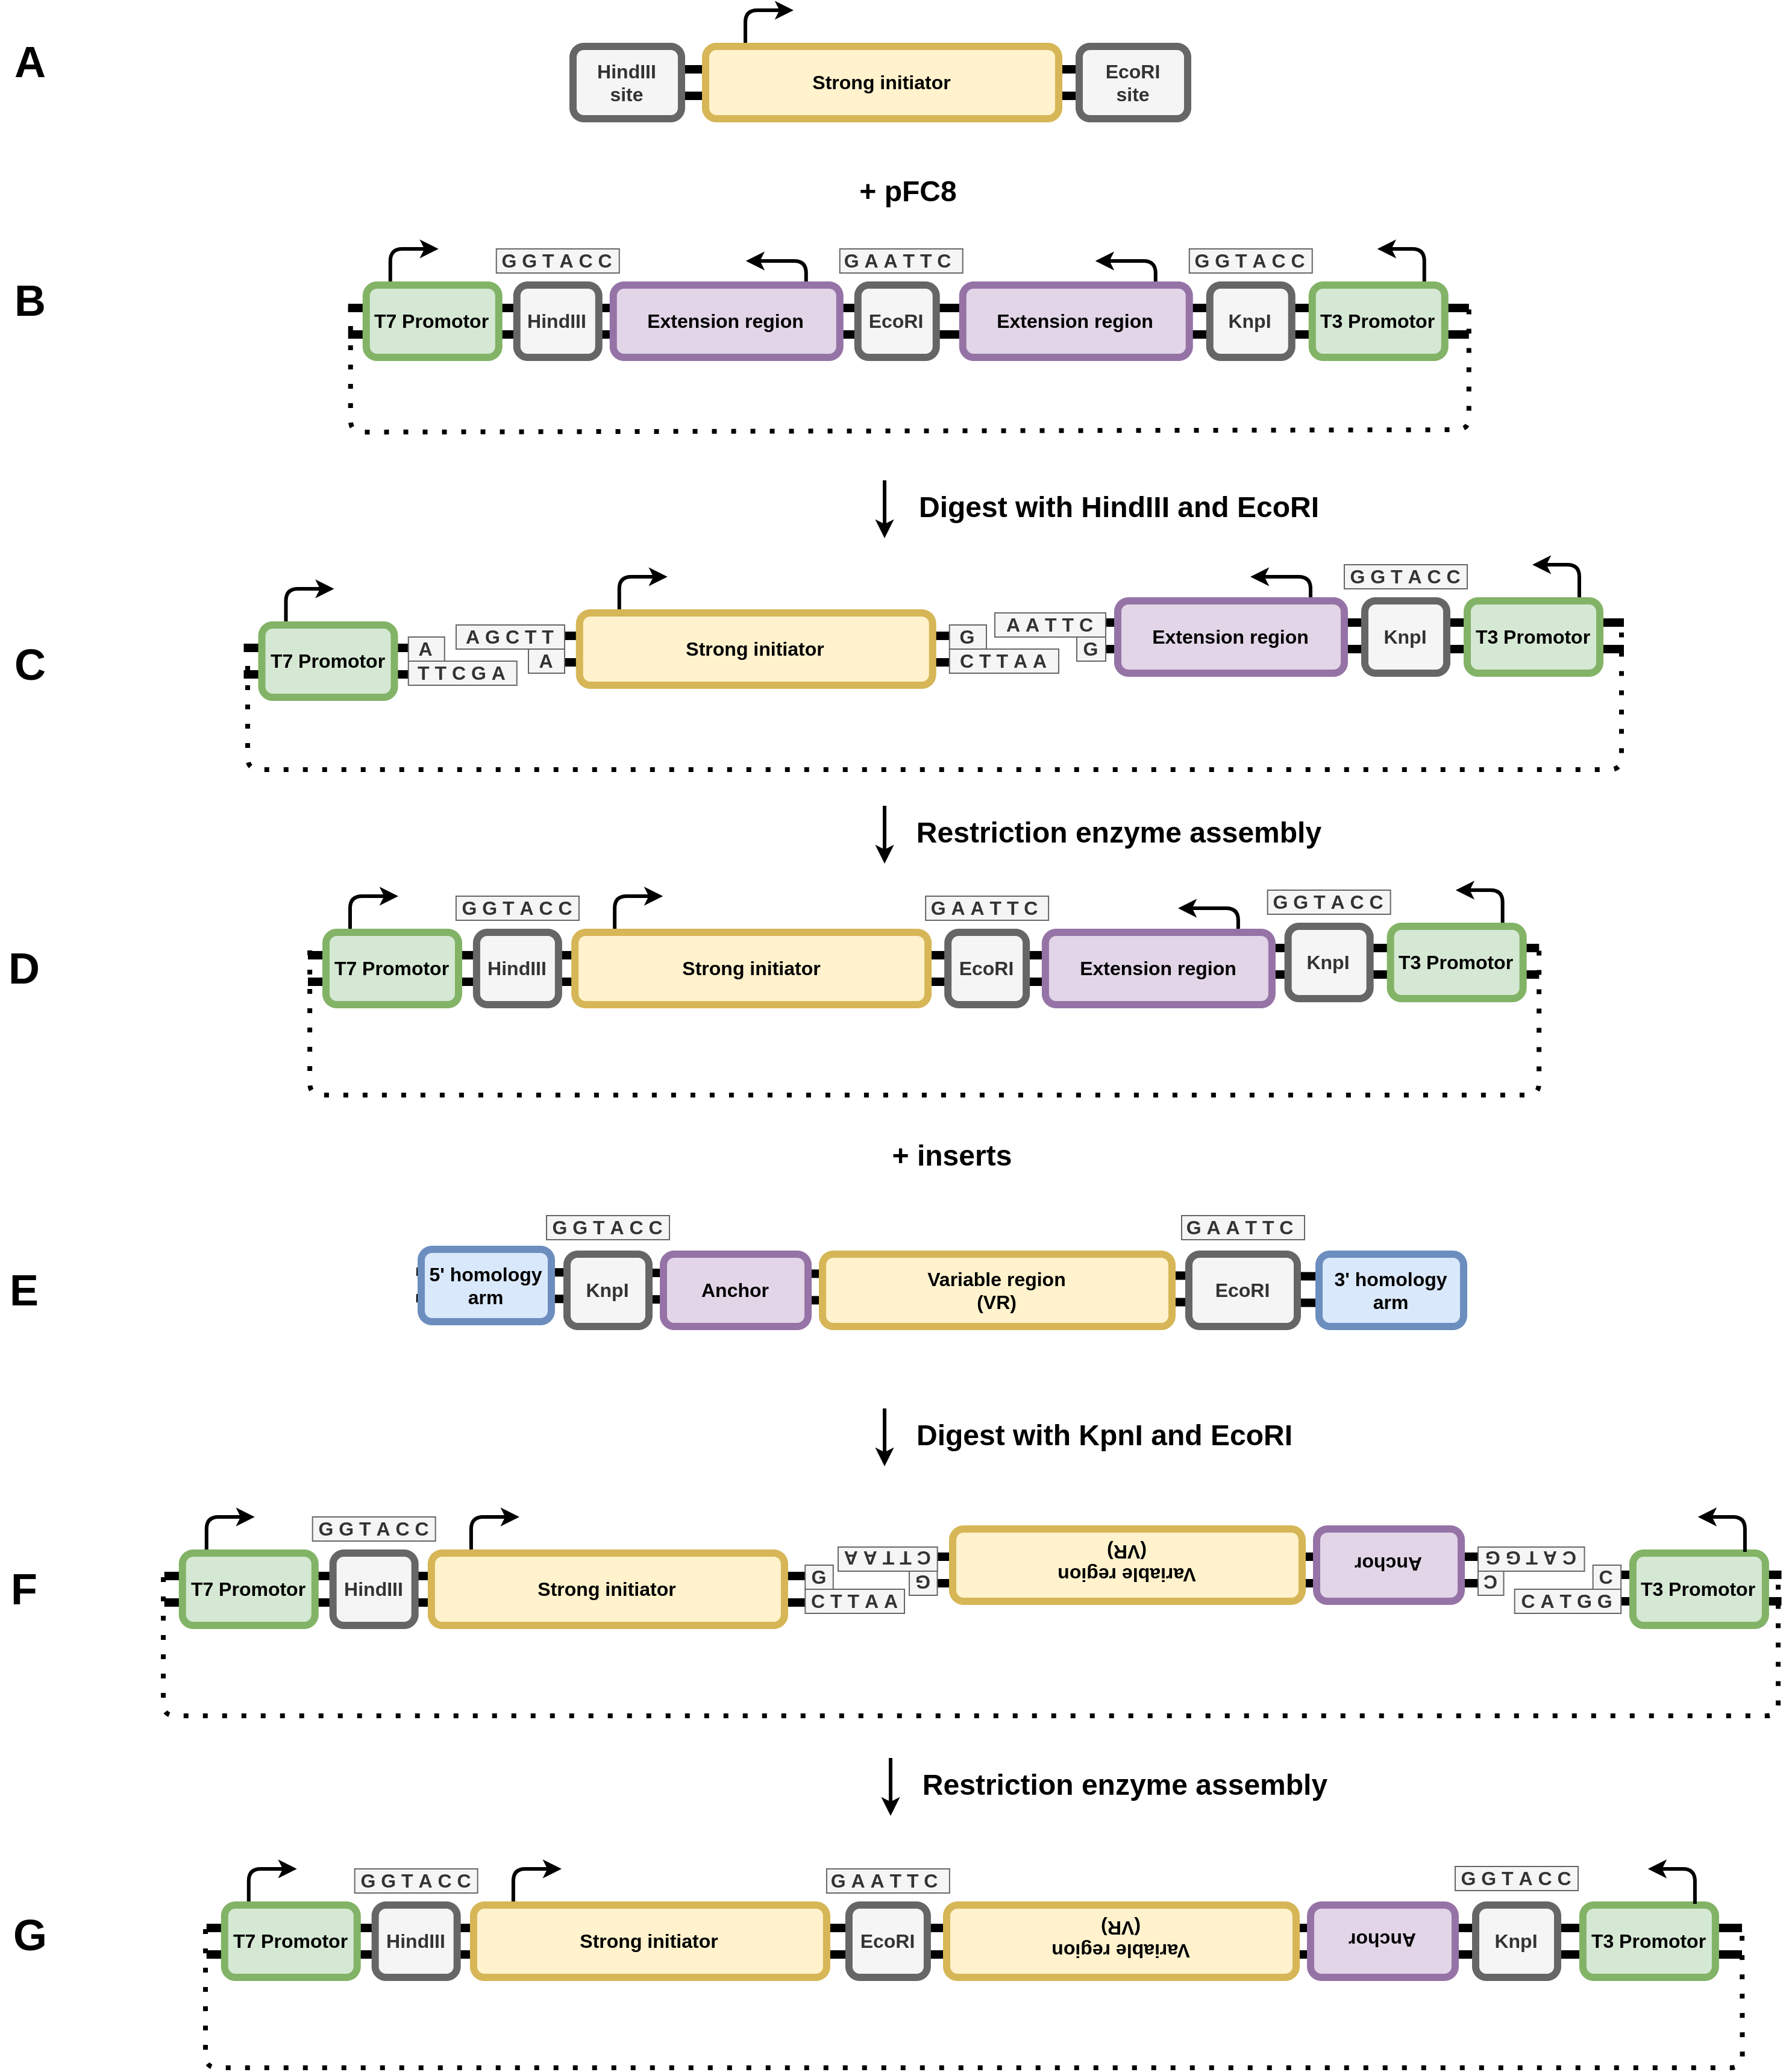
\includegraphics[width=15cm]{images/cloning_diagrams/construct_diagrams-T7-termination-series.png}
	\centering
	\caption{Diagram of pFC8 T7 termination series cloning strategy.}
	\label{clone:T7-term}
	
\end{figure}

 First, the strongest and most consistent R-loop initiator identified from the T7 initiation series will serve as the substrate for an additional synthetic double stranded DNA fragment containing the strong initiator sequence flanked by  HindIII and EcoRI recognition sequences (\ref{clone:T7-term}A). This strong initiator fragment will be added to pFC8  (\ref{clone:T7-term}B) and then the mixture digested with HindIII and EcoRI. The strong initiator will then anneal to the large pFC8 fragment via homology between the digested HindIII and EcoRI recognition sites (\ref{clone:T7-term}C). Next all termination inserts will be added to the pFC8-strong-initiator construct in equal molar ratios (\ref{clone:T7-term}D) and the mixture digested with KpnI and EcoRI (\ref{clone:T7-term}E). Inserts will then be incorporated into pFC8-strong-initiator constructs via homology between the digested KpnI and EcoRI sites (\ref{clone:T7-term}F). Since the order of these recognition sites on the pFC8-strong-initiator construct is opposite to that of the insert with respect to the T7 promoter the inserts will be present in the final construct in the reverse orientation and place the variable region downstream of the strong initiator (\ref{clone:T7-term}G). 
 
 \begin{figure}[H]
 	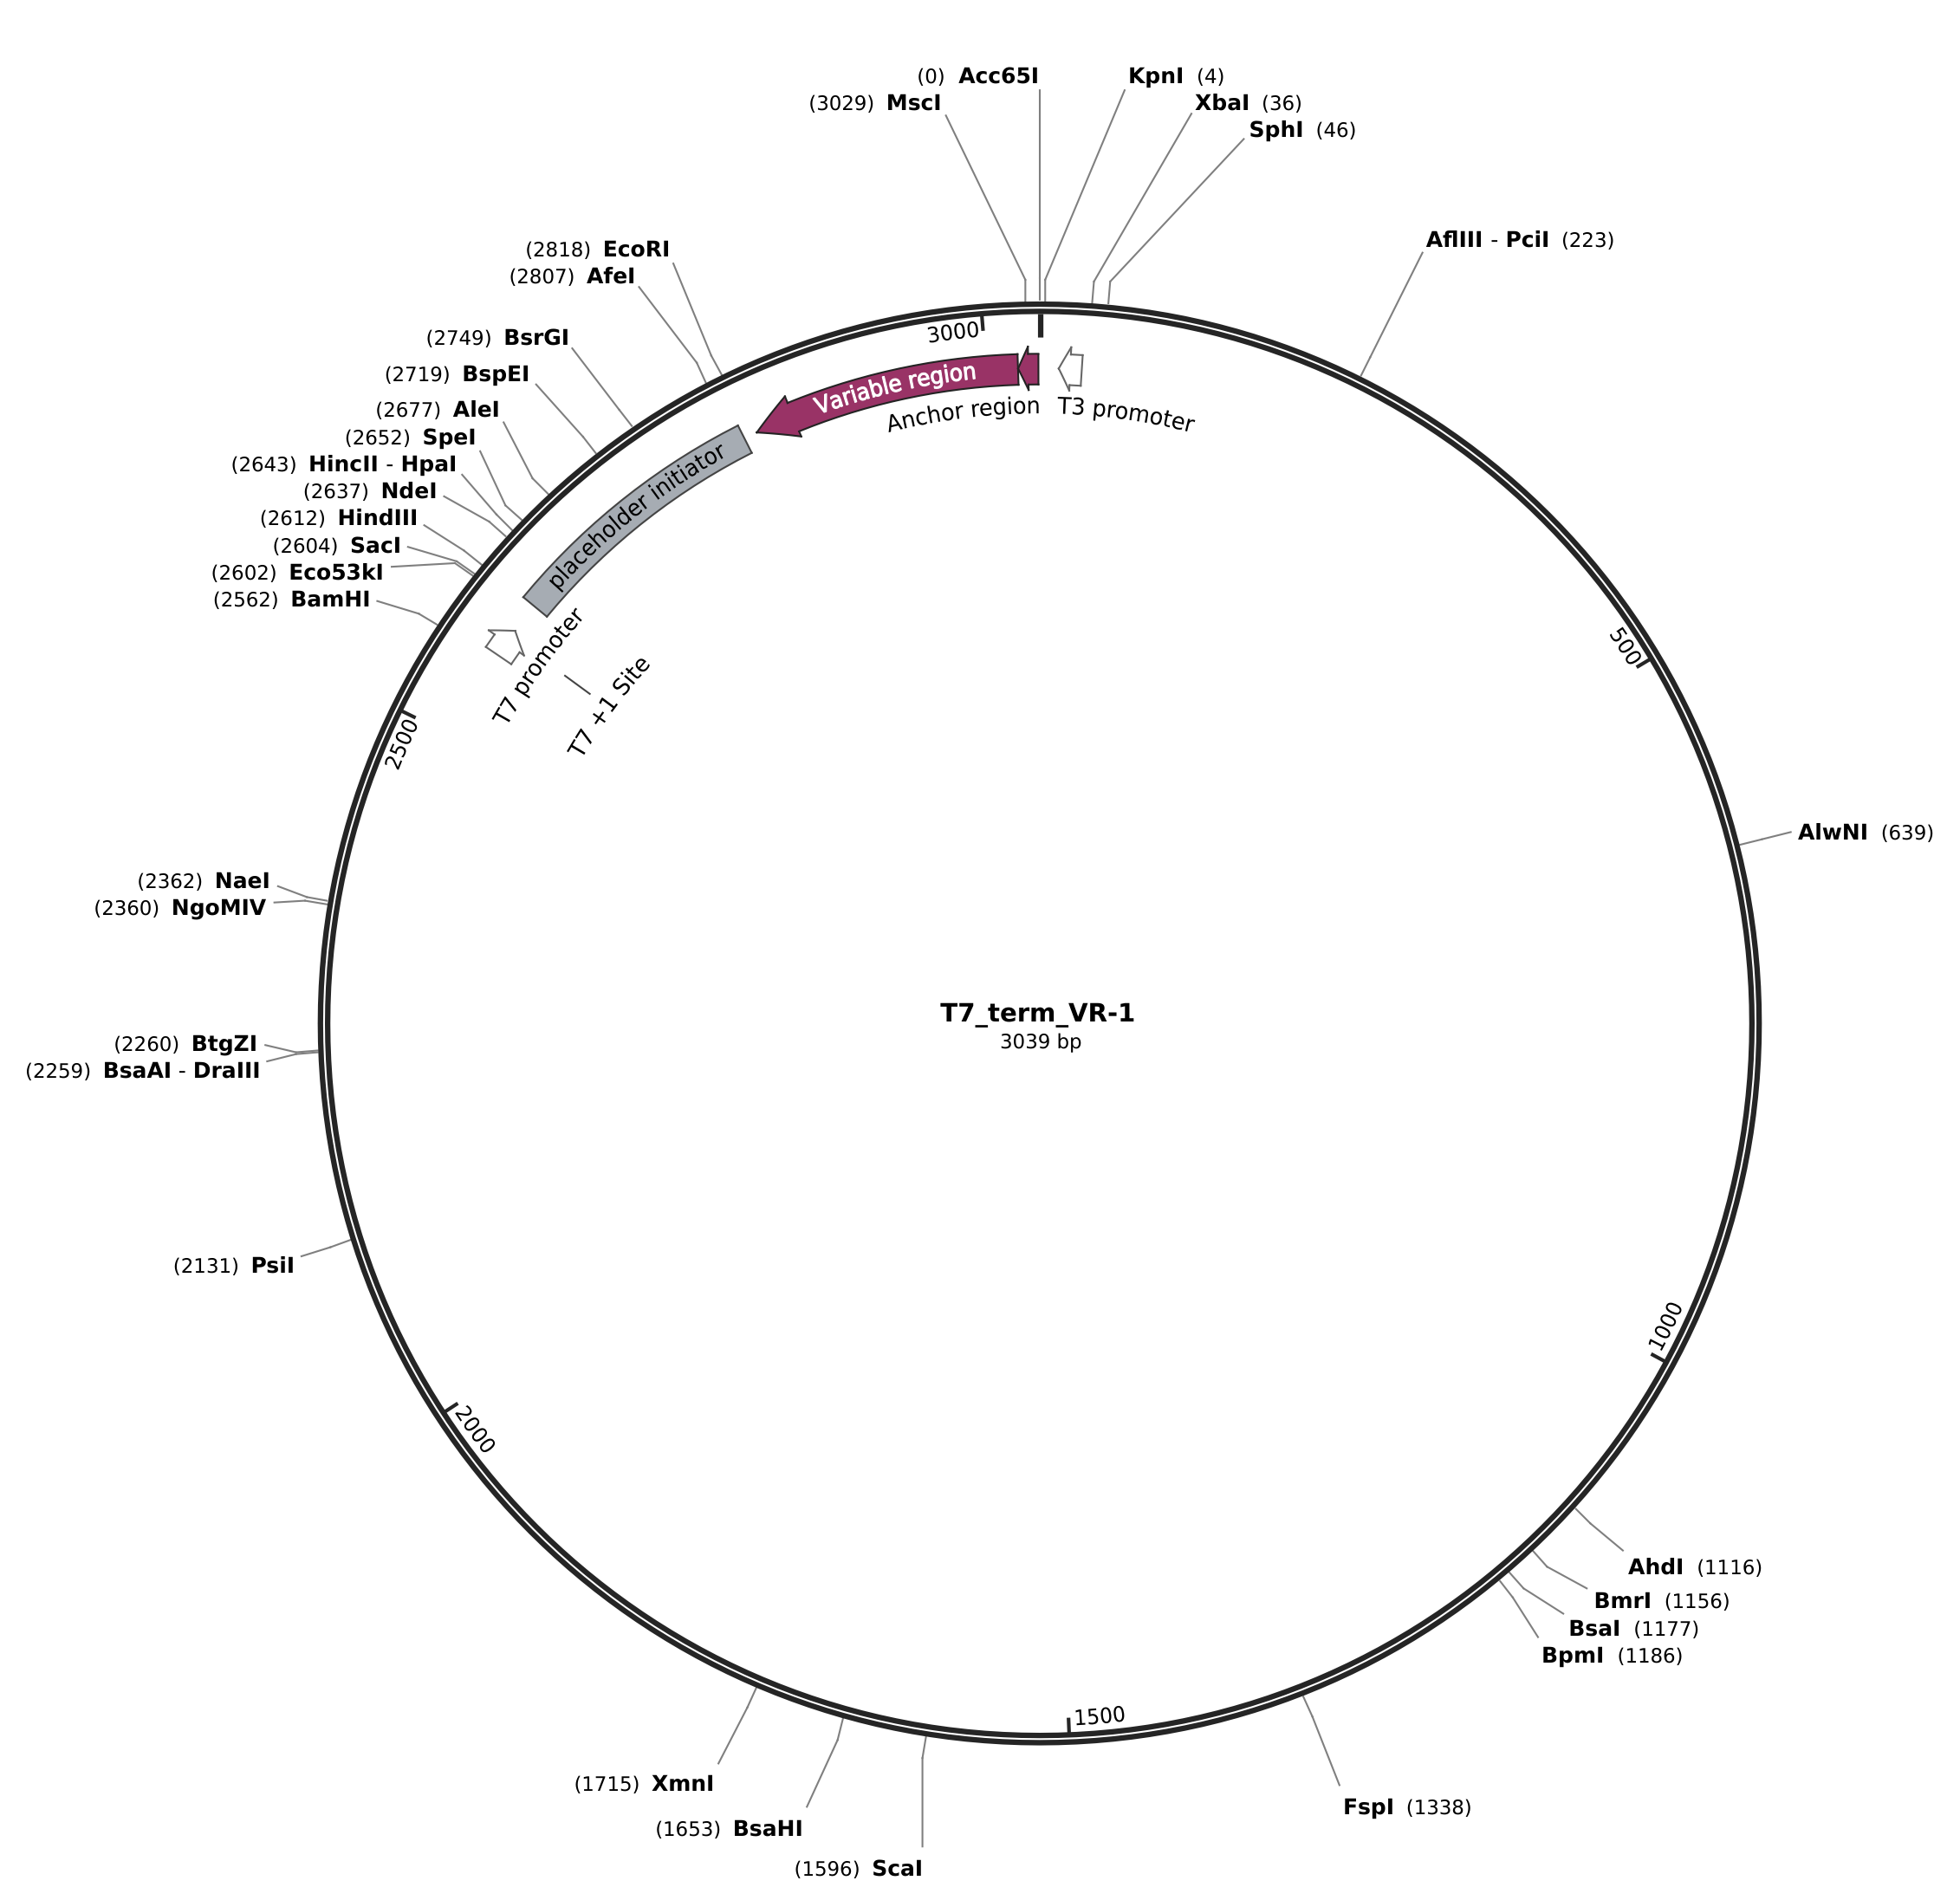
\includegraphics[width=12cm]{images/plasmid_maps/T7_term_VR-1 Map.png}
 	\centering
 	\caption{Plasmid map of produced by simulating the T7 termination series cloning protocol for the insert containing variable region 1. Cloning simulations were ran and confirmed to be successful for all complete inserts sequences. Note that since the strong initiation sequence that was used is to be determined a \href{https://github.com/EthanHolleman/plasmid-VR-design/blob/main/notes/placeholder_strong_initiator.ipynb}{simulated but functionally equivalent sequence} was used in its place.}
 	\label{clone:T7-term-insert-simulated}
 \end{figure}
 

\subsection{Tac initiation series constructs}
\label{sec:tac-init}

\begin{figure}[H]
	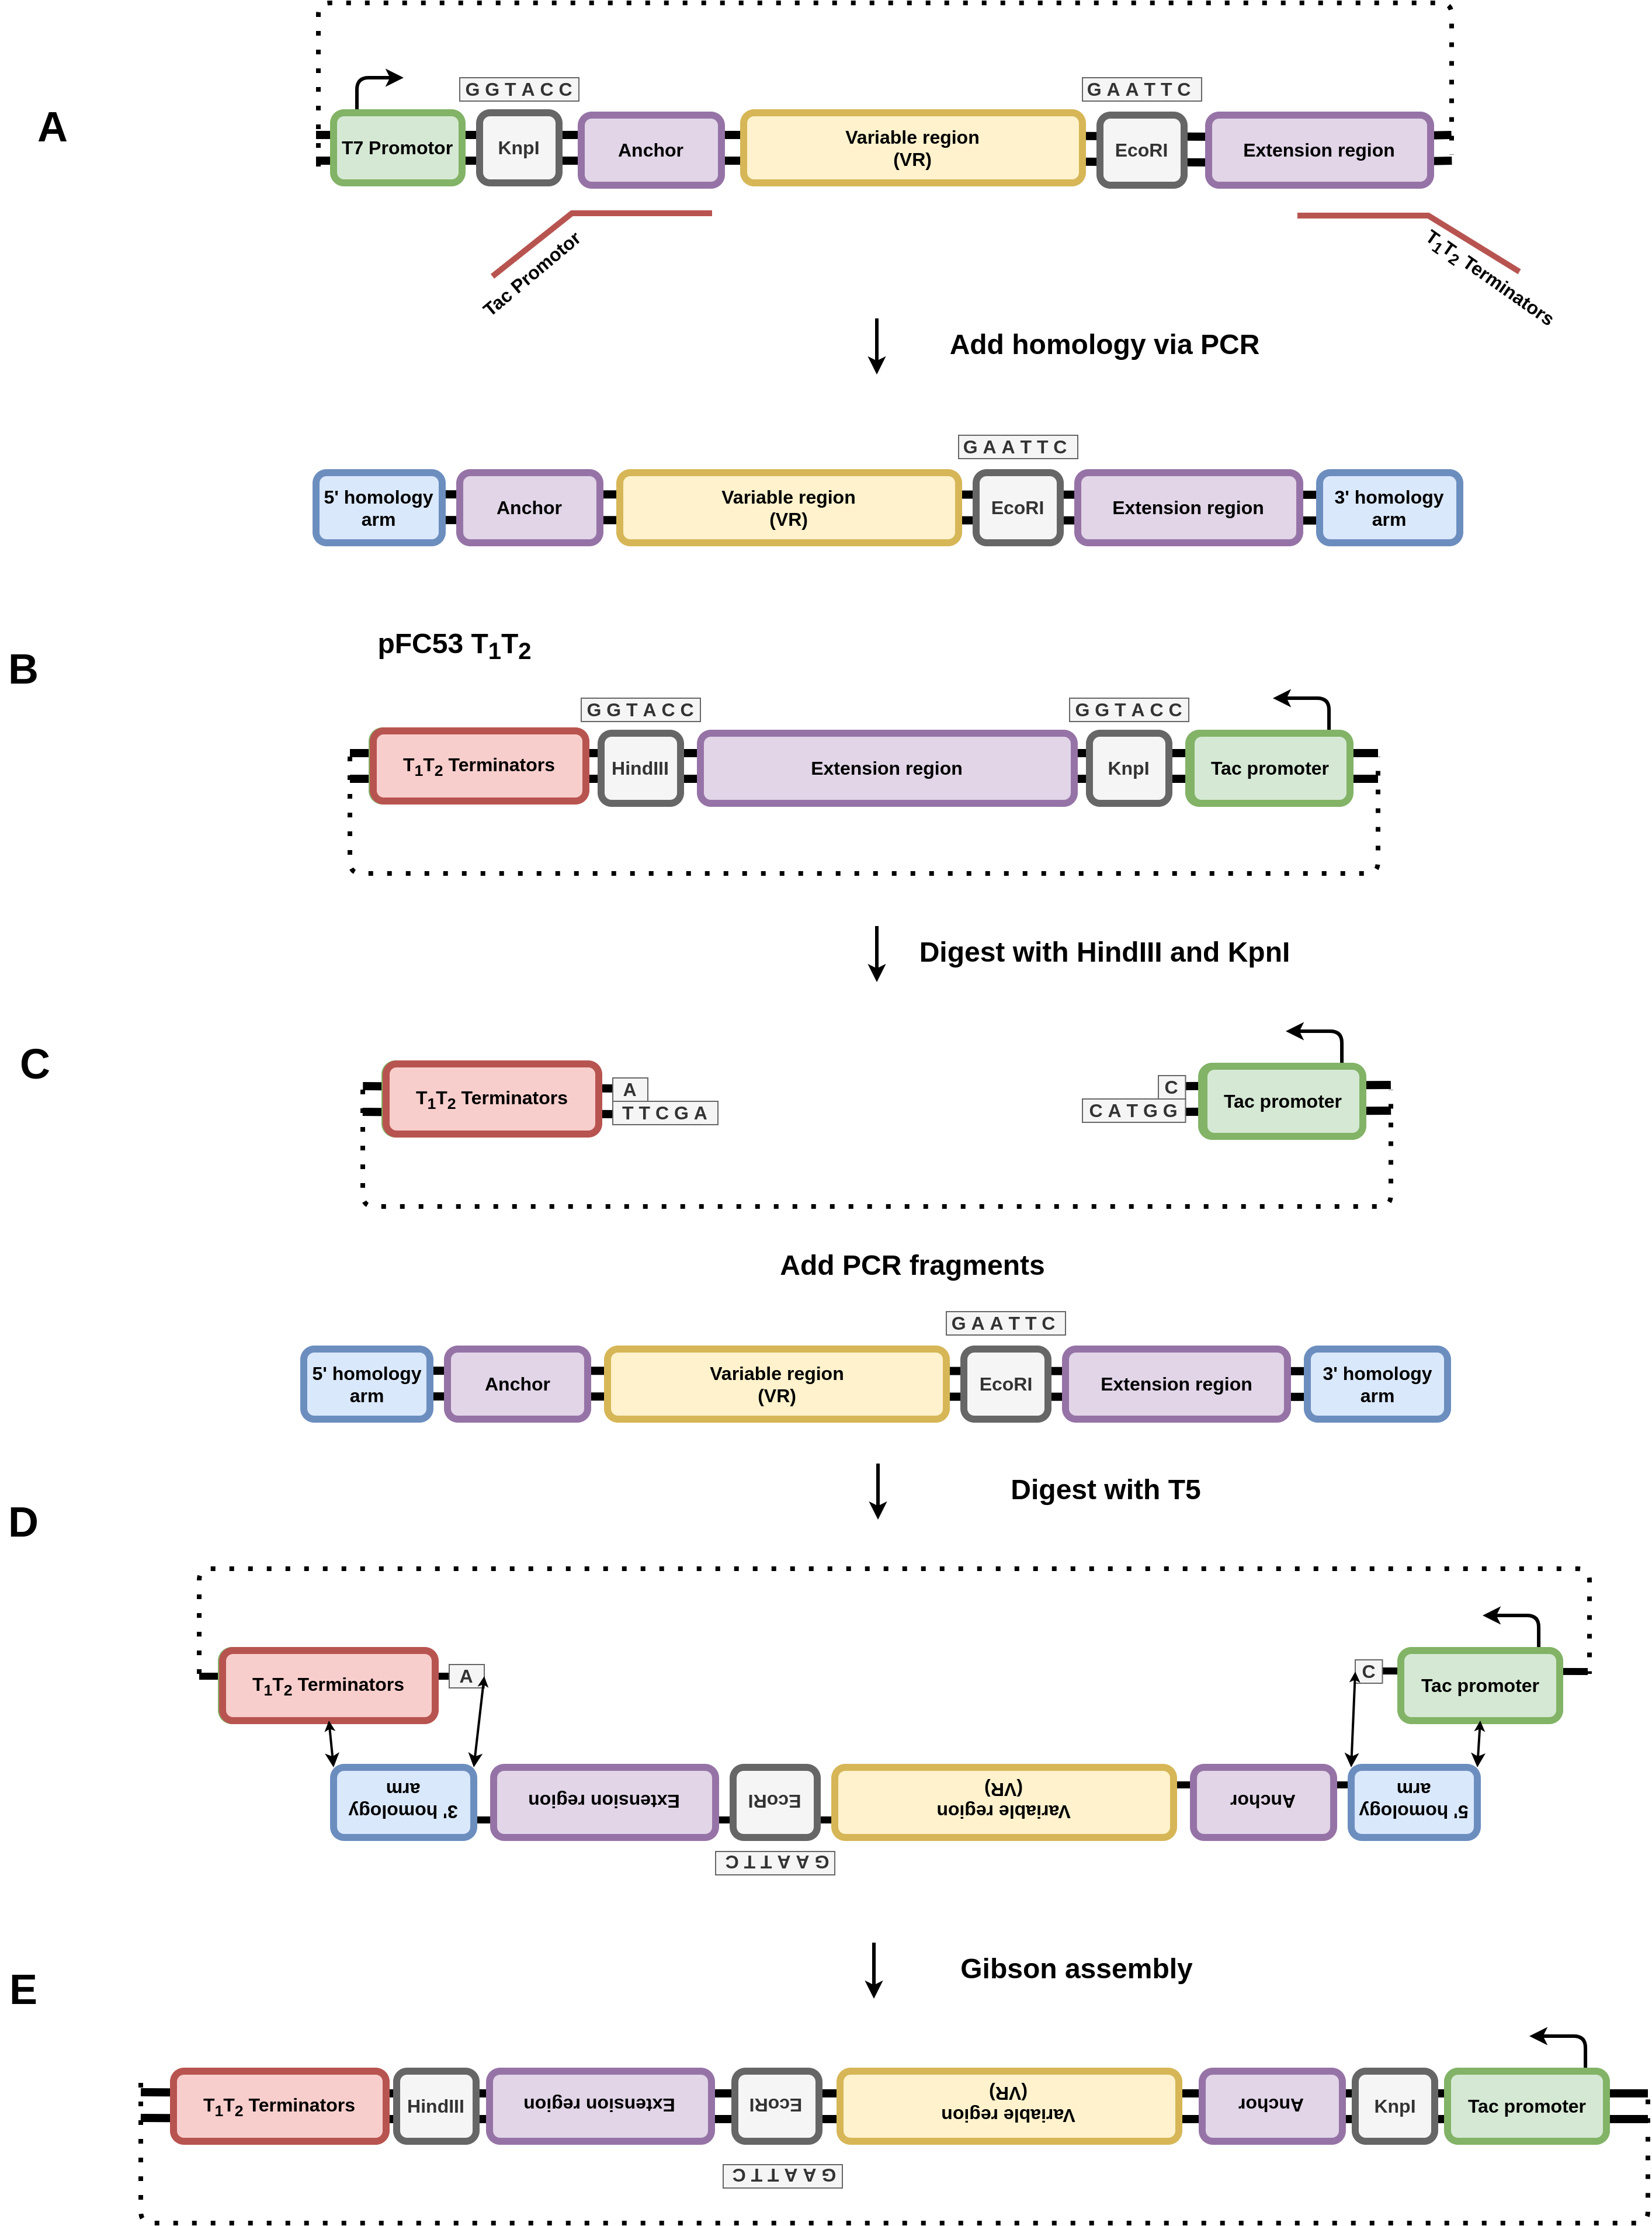
\includegraphics[width=15cm]{images/cloning_diagrams/construct_diagrams-Tac-initiation-series.png}
	\centering
	\caption{Diagram of pFCT$_1$T$_2$ tac initiation series cloning strategy.}
\end{figure}

First primers two pairs of primers are used to add amplify the anchor region, variable region, EcoRI recognition site and extension region from the T7 initiation construct library (\ref{sec:tac-init}). These primers will also contain overhangs with homology to the 5' end of the tac promoter and 3' T1T2 terminator sequences (\ref{T7:tac-init}A). Next, pFCT$_1$T$_2$ is separately digested with HindIII and KpnI and the large fragment is purified via agarose gel. The PCR products products are added to the large fragment and digested with T5 endonuclease (\ref{T7:tac-init}B, C). The final construct is assembled via Gibson assembly and the HindIII and KpnI sites are regenerated as a result of the insertion. 

\begin{figure}[H]
	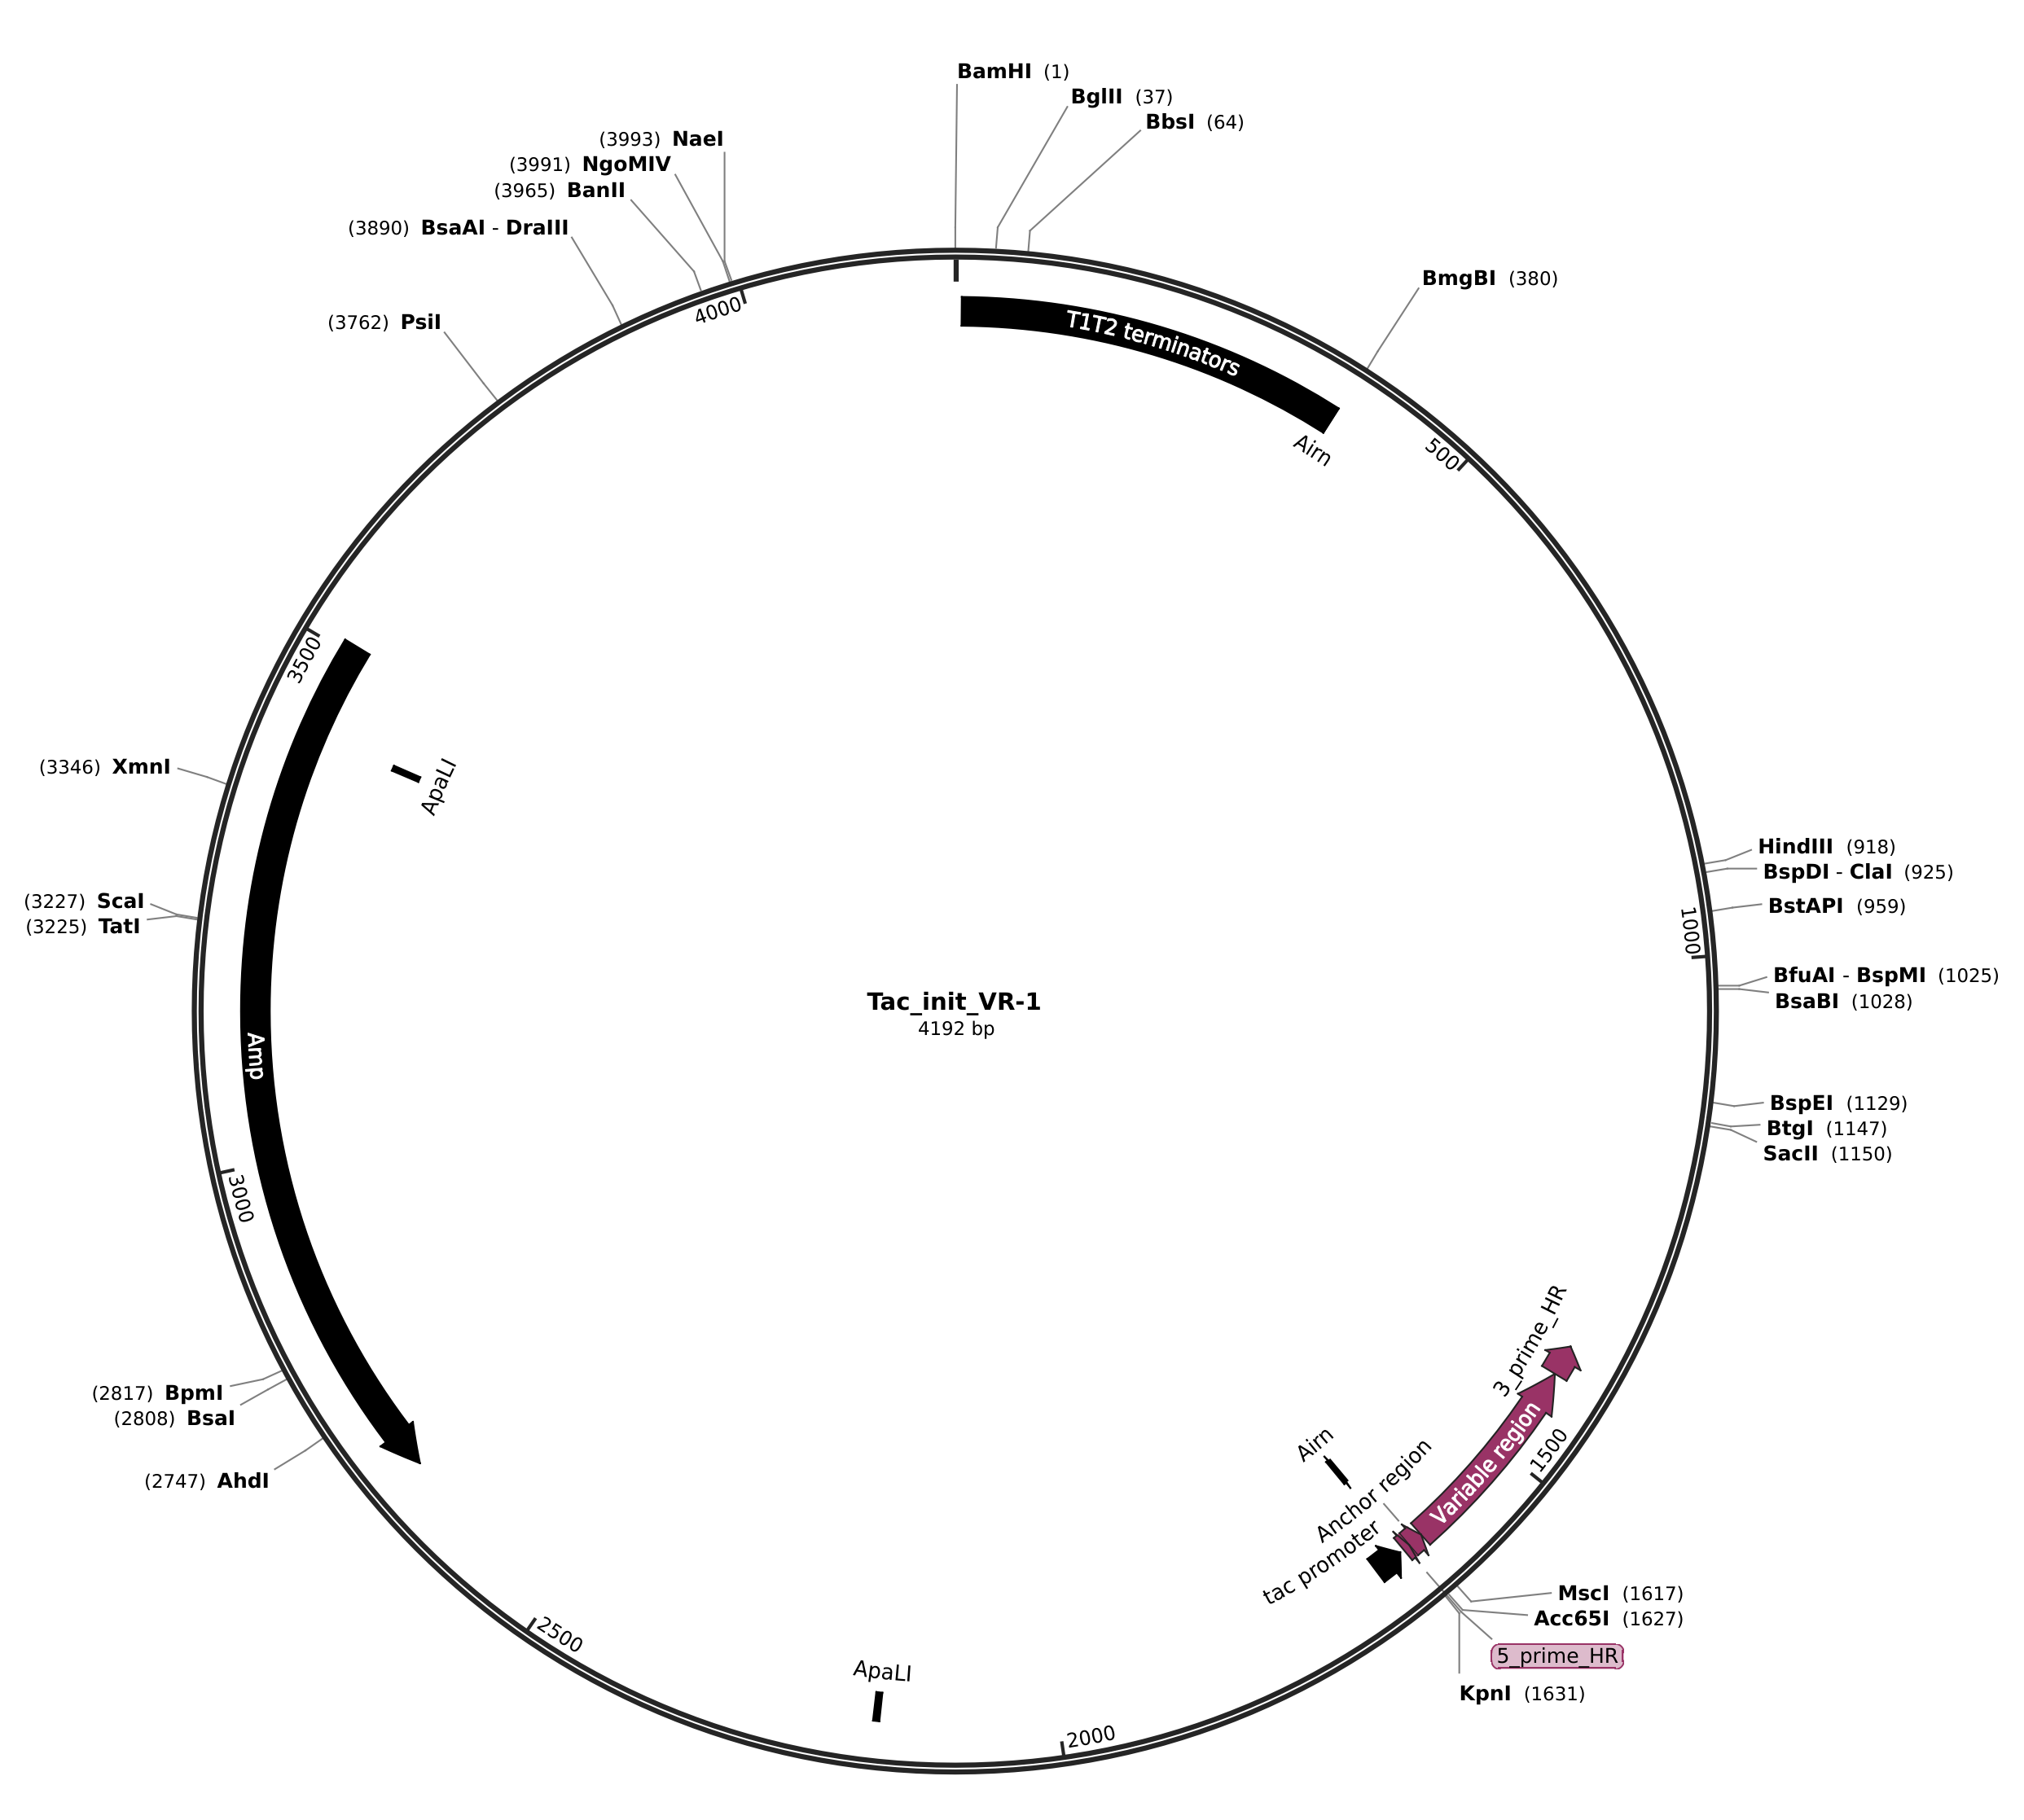
\includegraphics[width=15cm]{images/plasmid_maps/tac_init_simulated_assembly.png}
	\centering
	\caption{Plasmid map produced by simulating tac initiation series assembly protocols.}
\end{figure}


\subsubsection{Tac initiation series primer design}


\begin{figure}[H]
	\centering
	\begin{subfigure}[b]{\textwidth}
		\centering
		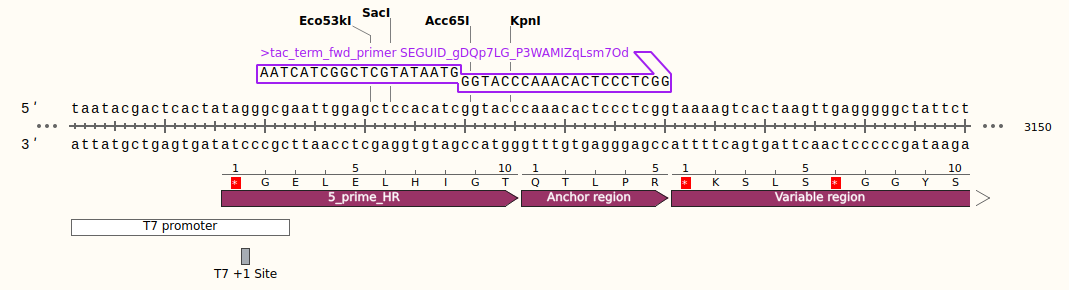
\includegraphics[width=0.75\textwidth]{images/primers/t7-init-forward.png}
		\caption{Forward primer. Targets the anchor region and adds homology to the downstream end of the Tac promoter of the pFC53T1T2 backbone and regenerates the digested KpnI site.}
		\label{fig:y equals x}
	\end{subfigure}
	\vfill
	\begin{subfigure}[b]{\textwidth}
		\centering
		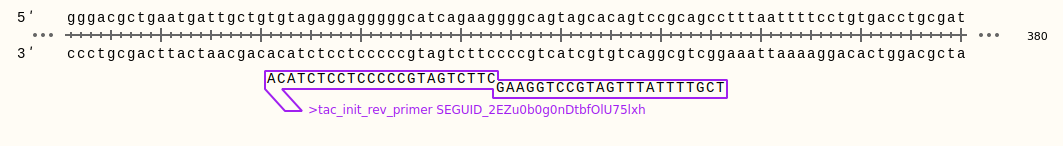
\includegraphics[width=0.75\textwidth]{images/primers/t7-init-reverse.png}
		\caption{Reverse primer. Targets an arbitrary region 500 nucleotides downstream of the end of the insert in order to include an "extension region" downstream of the variable region. Adds homology to the upstream end of the T1T2 terminator sequence of the pFC53T1T2 backbone and regenerates the digested HindIII site.}
		\label{fig:three sin x}
	\end{subfigure}
	\vfill
	\begin{subfigure}[b]{\textwidth}
		\centering
		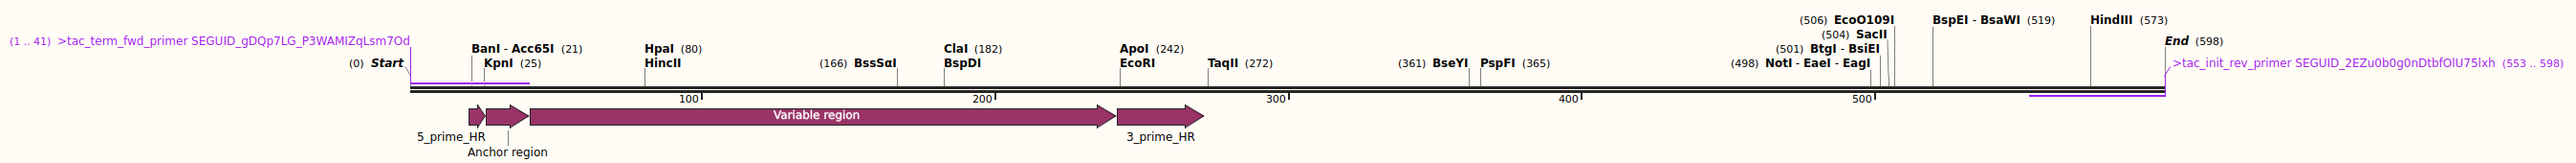
\includegraphics[width=0.75\textwidth]{images/primers/t7-init-amplicon.png}
		\caption{Amplicon produced by the forward and reverse primers.}
		\label{fig:three sin x}
	\end{subfigure}
	\caption{PCR primers and resulting amplicon used to produce tac initiation series constructs.}
\end{figure}


\begin{figure}[H]
	\centering
	\begin{BVerbatim}
	|95°C|95°C               |    |tmf:73.4
	|____|_____          72°C|72°C|tmr:78.5
	|5min|30s  \ 64.4°C _____|____|45s/kb
	|    |      \______/ 0:59|5min|GC 55%
	|    |       30s         |    |1318bp
	\end{BVerbatim}
	\caption{PCR program for Tac polymerase for tac initiation series primers.}
\end{figure}


\subsection{Tac termination series constructs}
\label{sec:tac-termination}

The assembly protocol for the tac termination series is identical to the initiation series, the difference being the insert is sourced from T7 termination series constructs and accordingly a different set of primers is utilized to amplify the insert region and add homology for Gibson assembly into 
pFCT$_1$T$_2$.

\begin{figure}[H]
	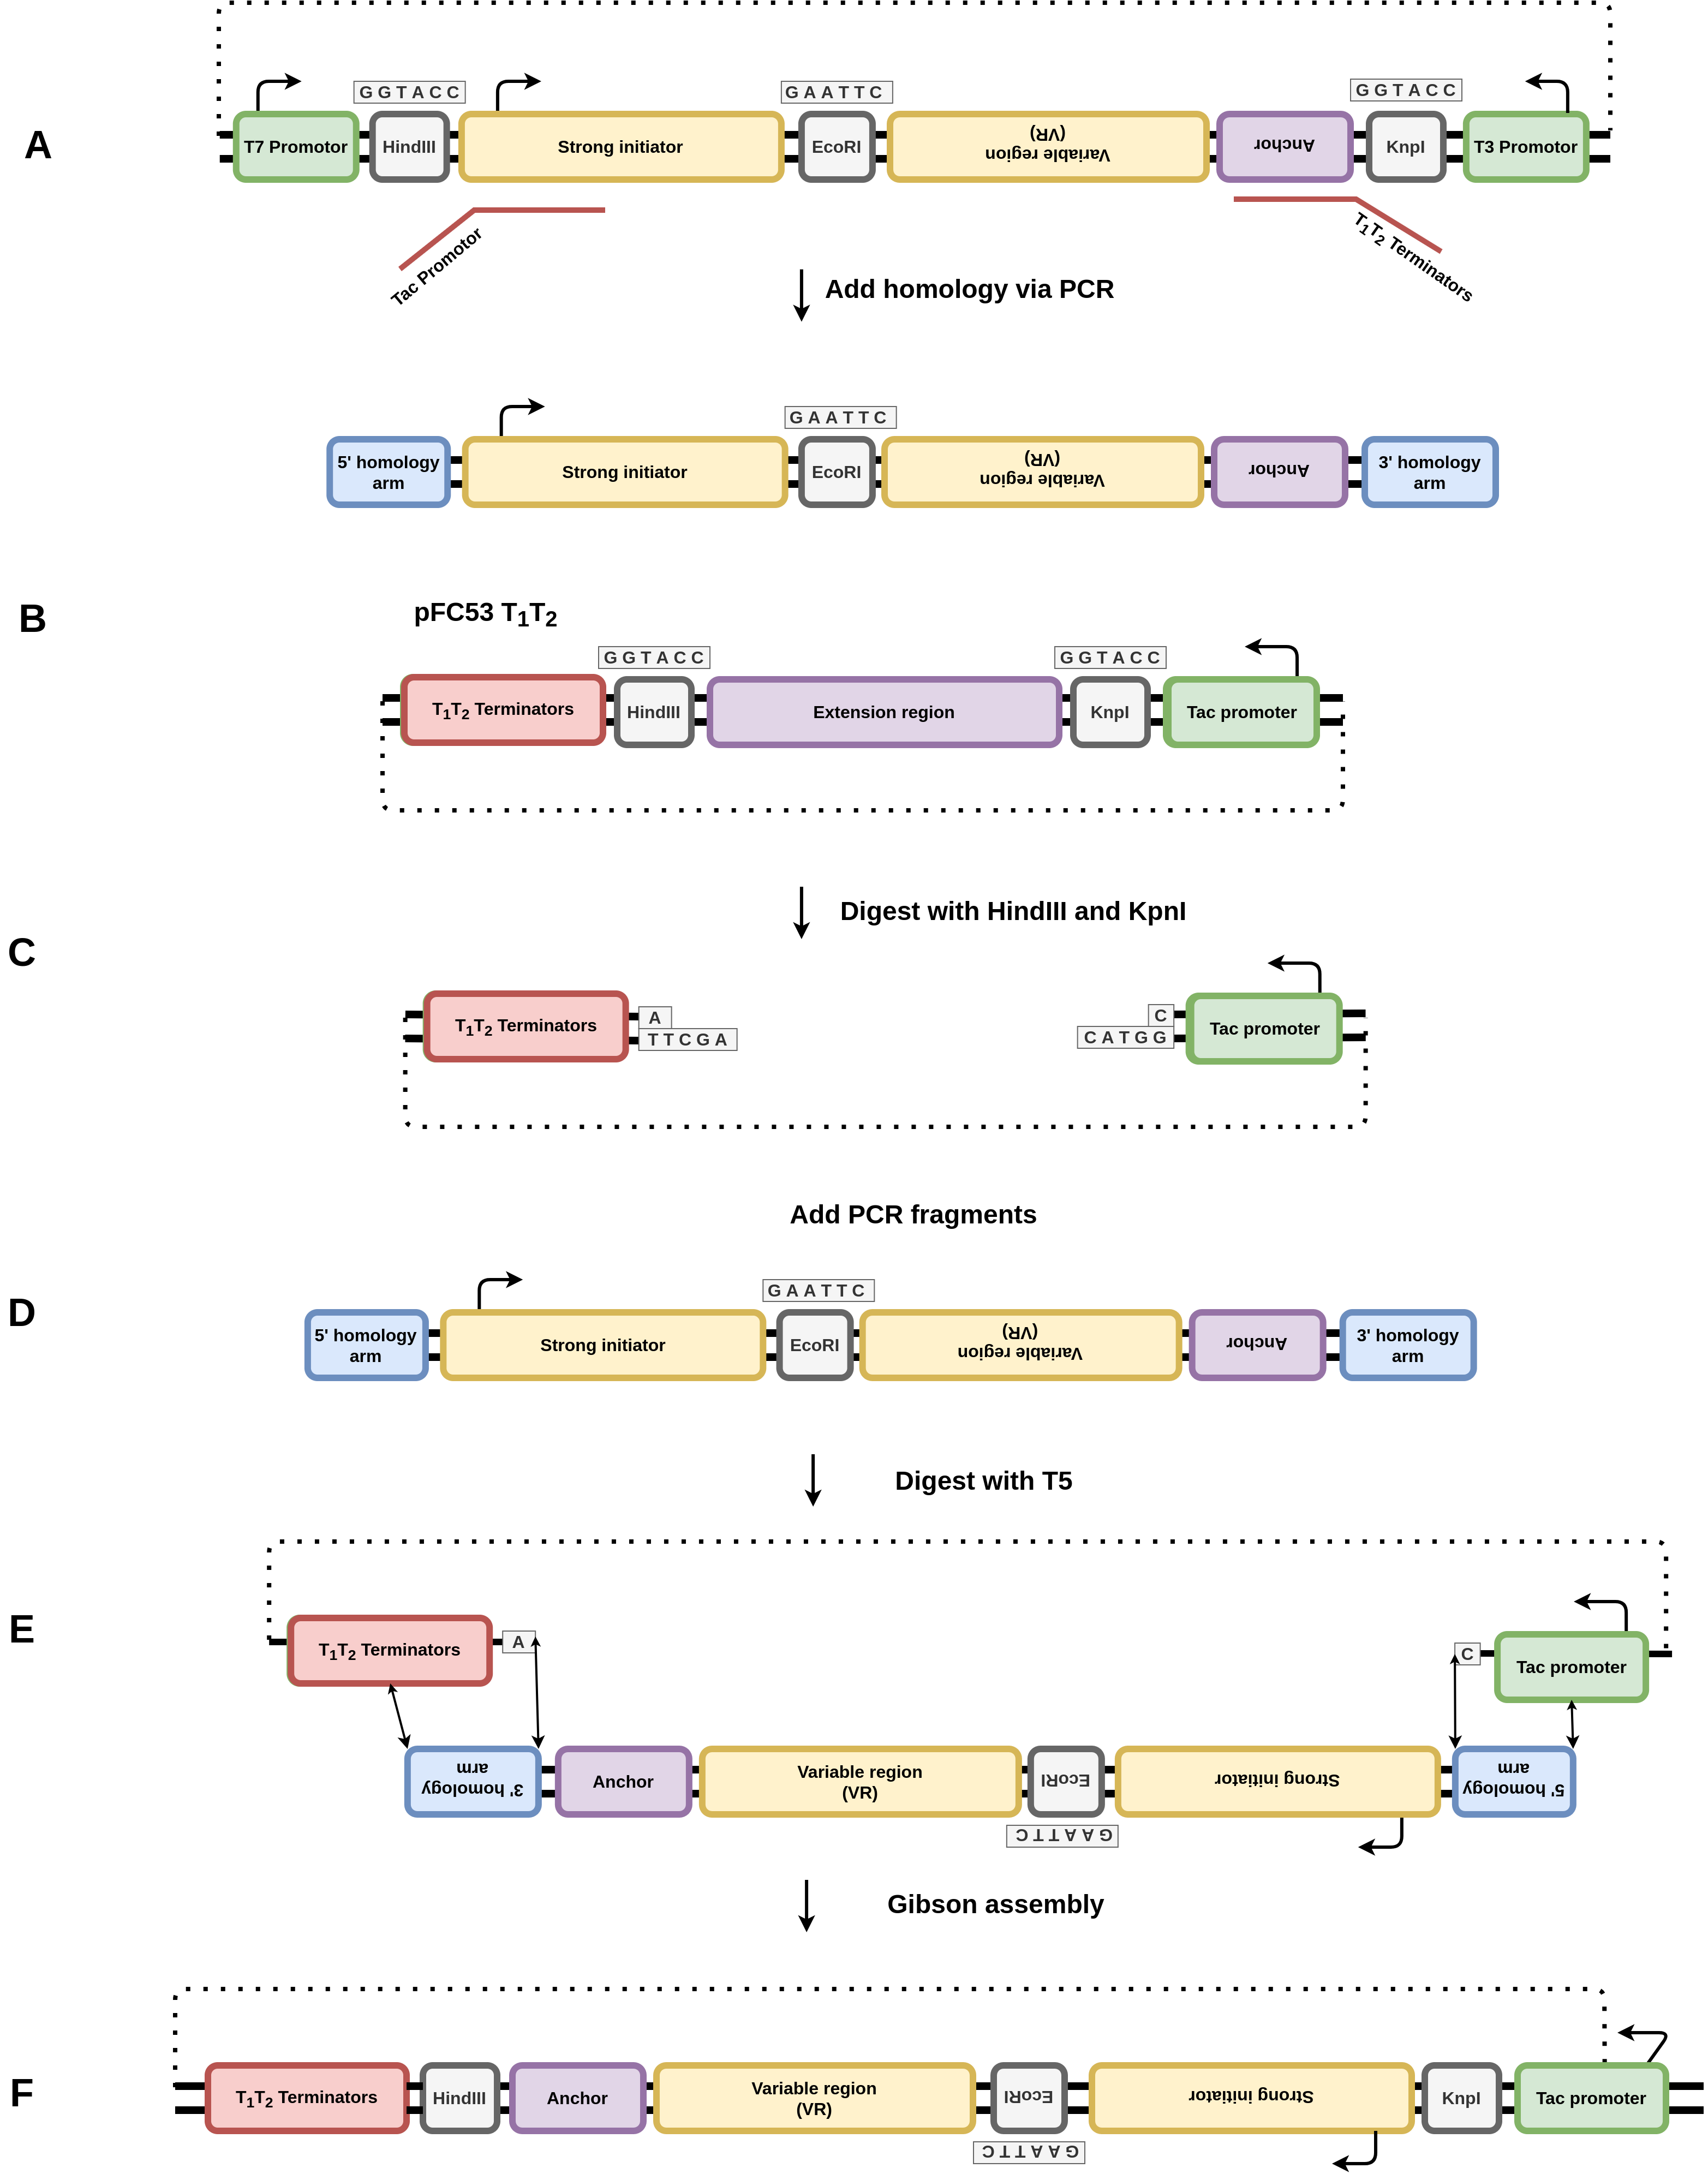
\includegraphics[width=15cm]{images/cloning_diagrams/construct_diagrams-Tac-termination-series.png}
	\centering
	\caption{Diagram of pFCT$_1$T$_2$ termination series cloning strategy.}
\end{figure}

\begin{figure}[H]
	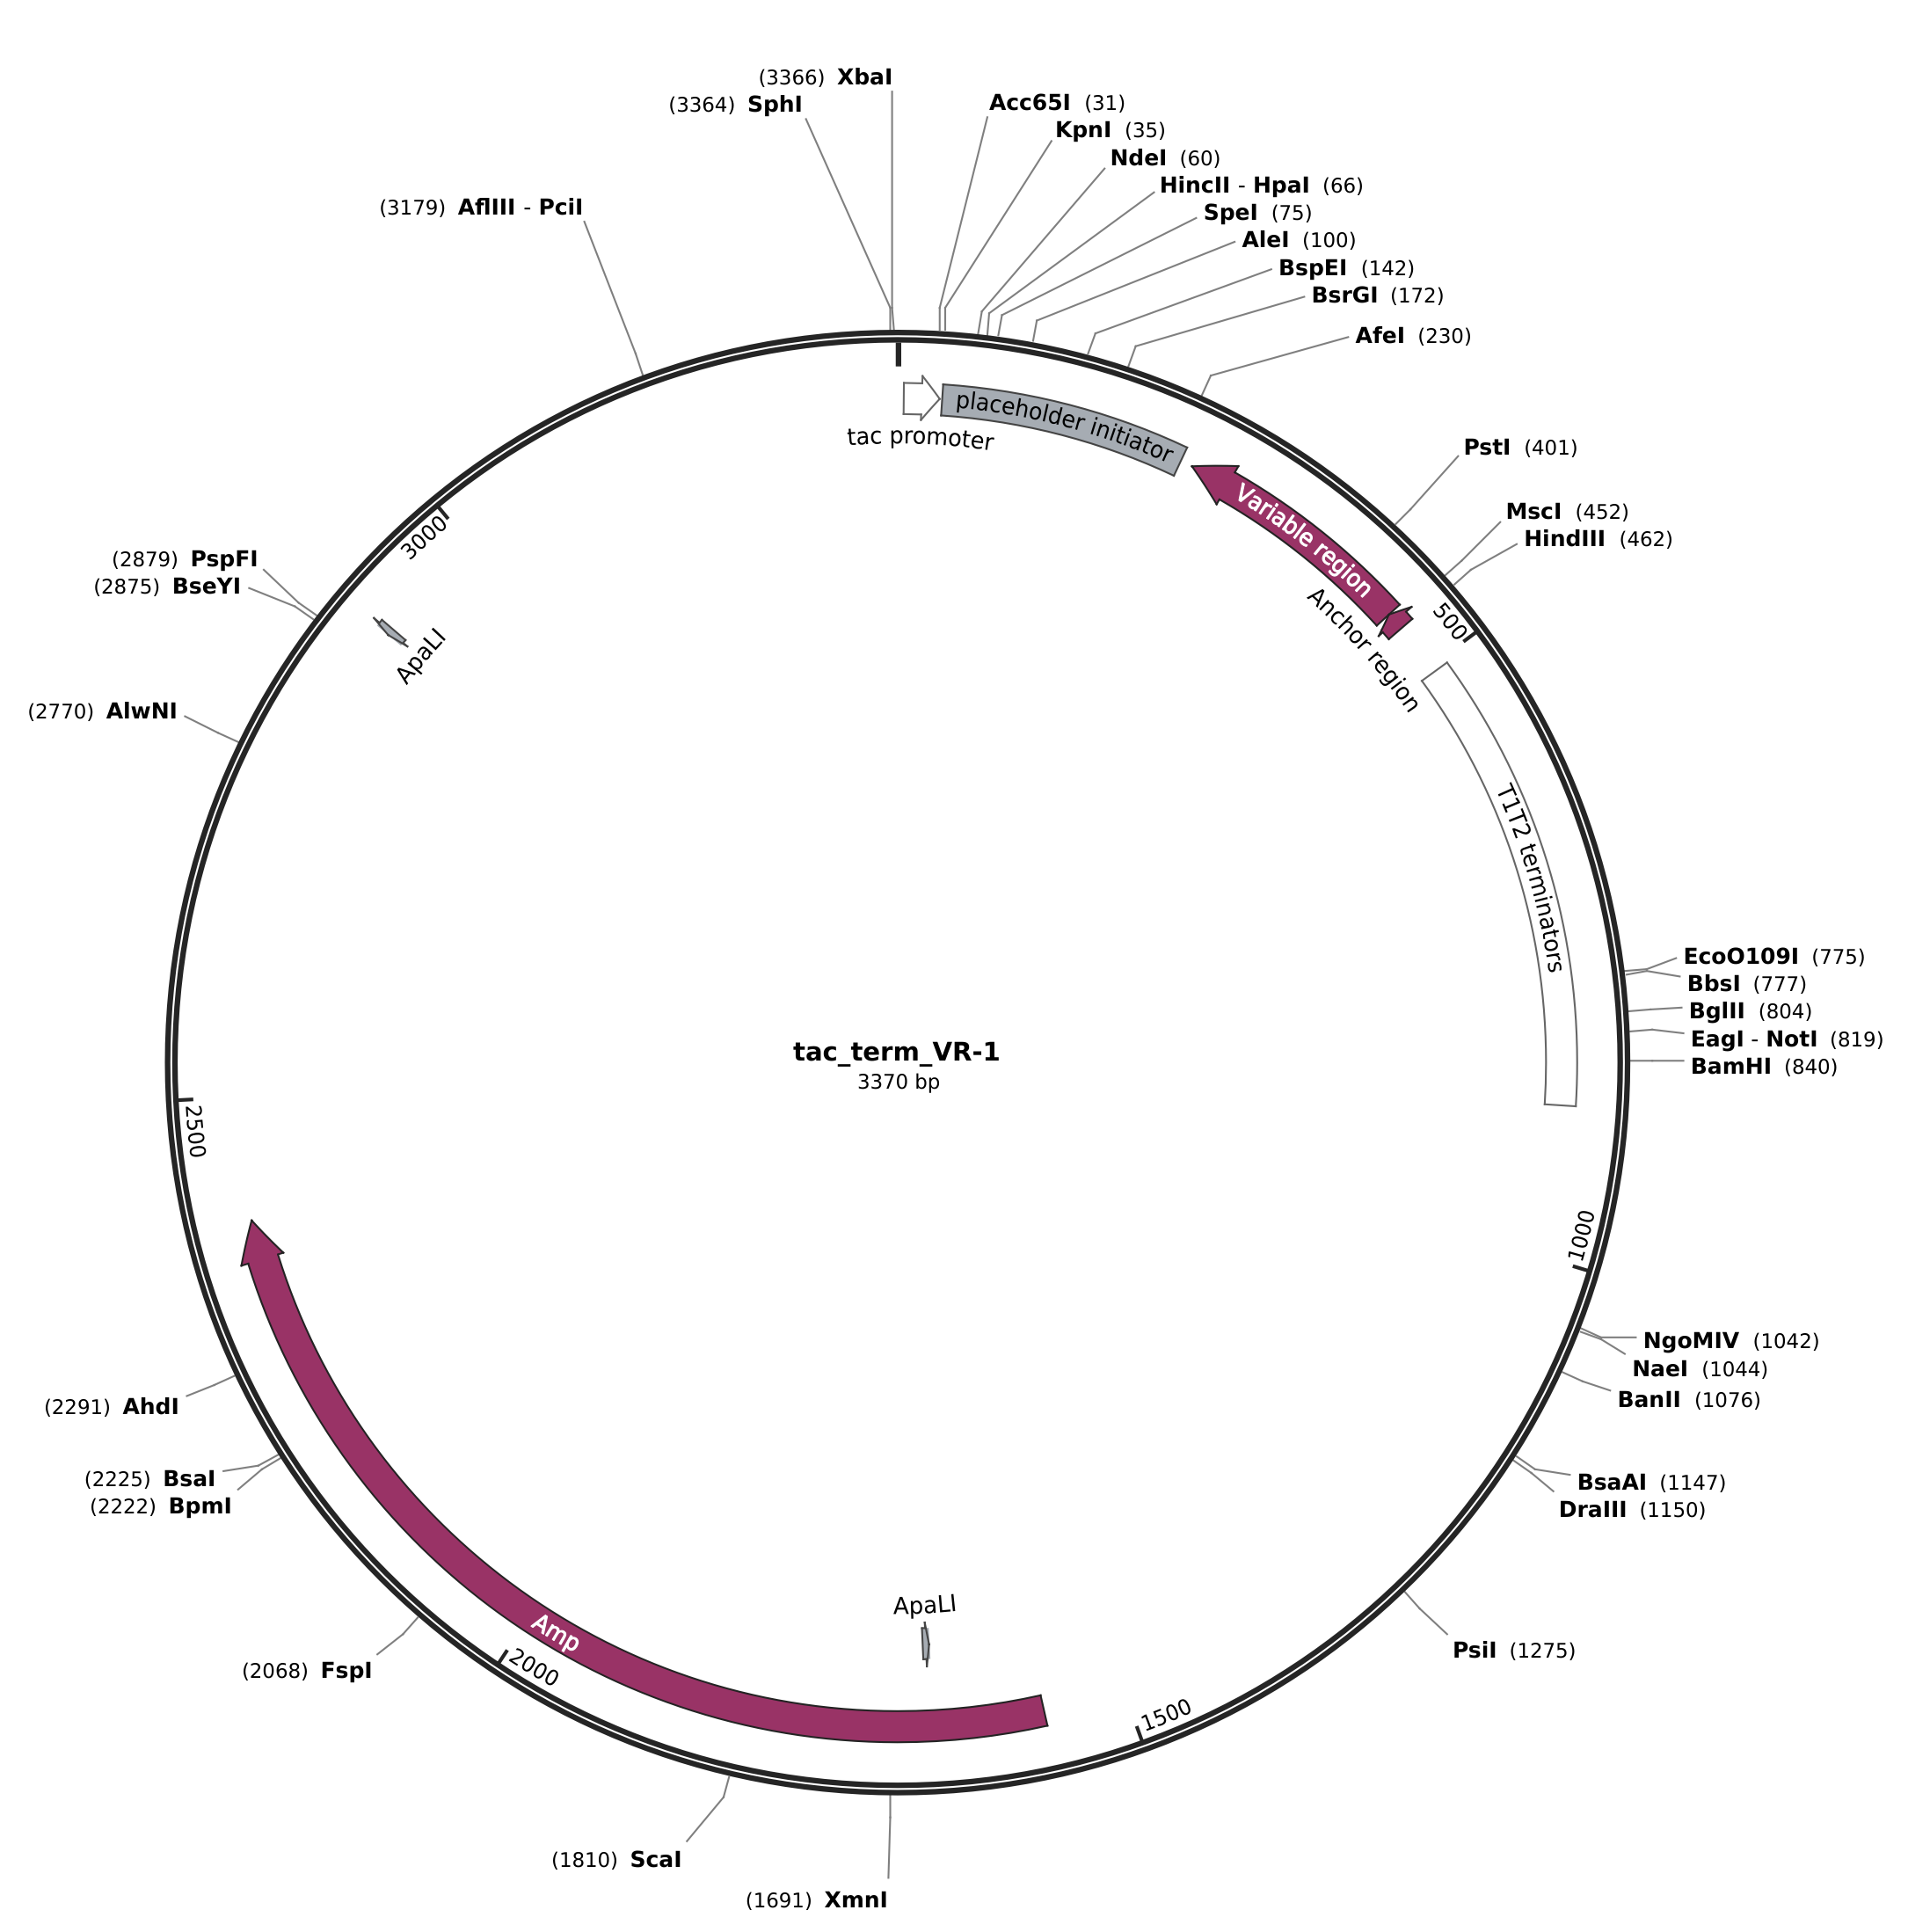
\includegraphics[width=15cm]{images/plasmid_maps/tac_term_simulated_assembly.png}
	\centering
	\caption{Plasmid map produced by simulating tac termination series assembly protocols.}
\end{figure}

\subsubsection{Tac termination series primer design}

\begin{figure}[H]
	\centering
	\begin{subfigure}[b]{\textwidth}
		\centering
		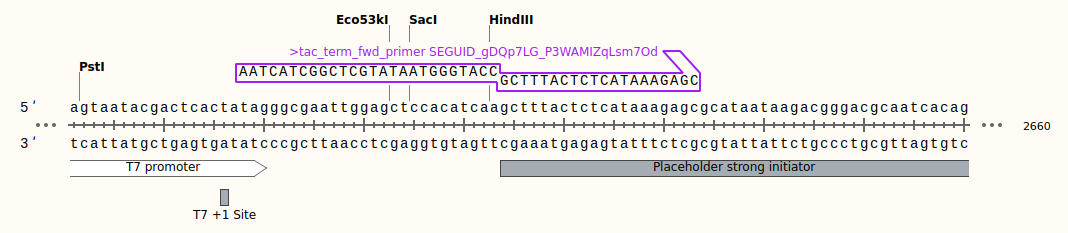
\includegraphics[width=0.75\textwidth]{images/primers/t7-term-forward.png}
		\caption{Forward primer. Targets the 5' end of the placeholder strong initiator and adds homology to the downstream end of adds homology to the downstream end of the Tac promoter of the pFC53T1T2 backbone and regenerates the KpnI site.}
		\label{fig:y equals x}
	\end{subfigure}
	\vfill
	\begin{subfigure}[b]{\textwidth}
		\centering
		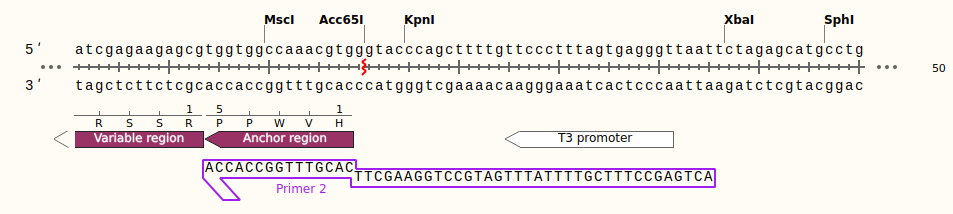
\includegraphics[width=0.75\textwidth]{images/primers/t7-term-reverse.png}
		\caption{Reverse primer. Targets the anchor region and adds homology to the to the upstream end of the T1T2 terminator sequence of the pFC53T1T2 backbone and regenerates the HindIII site.}
		\label{fig:three sin x}
	\end{subfigure}
	\vfill
	\begin{subfigure}[b]{\textwidth}
		\centering
		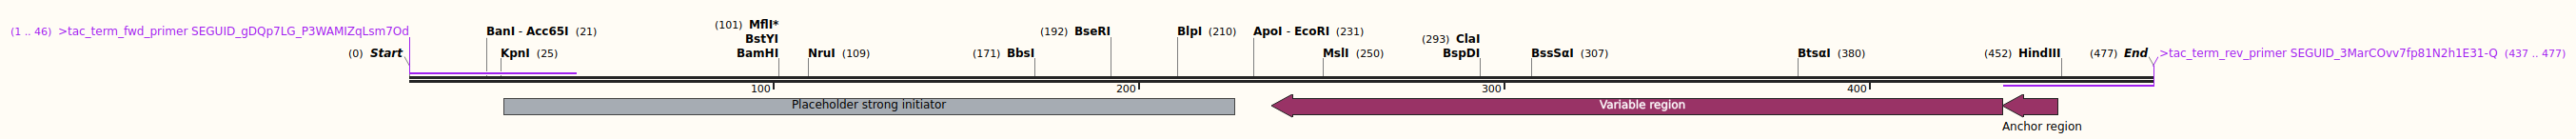
\includegraphics[width=0.75\textwidth]{images/primers/t7-term-amplicon.png}
		\caption{Amplicon produced by the forward and reverse primers.}
		\label{fig:three sin x}
	\end{subfigure}
	\caption{PCR primers and resulting amplicon used to produce tac termination series constructs.}
\end{figure}


A PCR program is not included here as an placeholder initiation region was used to demonstrate how tac termination series primers would be designed. Therefore until an actual strong initiator region is determined and verified these primers should \emph{not} be ordered. Code to generate both initiation and termination series primers and PCR programs is available as a Jupyter notebook \href{https://github.com/EthanHolleman/plasmid-VR-design/blob/main/notes/tac_series_primers.ipynb}{at this link}. This was later converted into a functionally equivalent notebook that is run as part of the insert calculation pipeline. 


\subsection{Validation of insert libraries}

Since all inserts of a given series will be assembled into their respective backbone in the same pot, it will be necessary to confirm that each insert-backbone assembly are present in relatively equal concentrations in the final library. Since the variable region of each insert-backbone assembly will be unique, qPCR utilizing primers that target a subset or all variable regions can be utilized to measure relative insert-backbone concentrations in the library. Potential primers for each insert are available at this link. 

\subsection{Quantification of R-loop formation }

Short description of SMRF-seq protocol using barcoded PCR primers for amplification 
and anticipated data analysis. 

\subsection{Reagents and kits}

\begin{itemize}
	\item \href{https://www.neb.com/products/e2611-gibson-assembly-master-mix#Product\%20Information_Properties\%20\&\%20Usage}{NEB Gibson assembly master mix}
	\item \href{https://www.neb.com/products/m0491-q5-high-fidelity-dna-polymerase#Product\%20Information}{NEB High-Fidelity DNA Polymerase}
	\item \href{https://www.qiagen.com/us/products/discovery-translational-research/dna-rna-purification/dna-purification/dna-clean-up/qiaquick-gel-extraction-kit/#orderinginformation/}{QIAquick gel extraction kit}. 
	\item \href{https://www.neb.com/products/r0176-dpni?__cf_chl_jschl_tk__=d22d8cb49b9b2d4ff2532de61875fea36af4066f-1626291600-0-ARBMmni5PdhcCrqckk9zN05YGR50cB-otICbDTrUStRYlPQzdrbyJvjEOoI2QusMU-HOcKBcontIQfQRYoQqN9R2hNCL0XzFa2hP3-_c6Vf1sL2Sb2Bs_DXW38t8Oc1NxSg0caQ4FlAGqVNswAJaml9BhLC5dWj1sCuqKwDj72JKO8eI9d3mlCcNVIAVs8n1xFpuo1_oyafffkTnQ-ysv358pg1RrIbChfkwqXctDQennQm_CRjVjuitrXFFNjgAqBDJBKFRMZKkoOYlTDEDBsuaQaQtMxNwL5u7yIJ5mNCrkkuiikIGg7Was3tNj1d7D-7bnJrfXr8jIfG3qW6kvIkrZBJey0JQAVMQGVc4Ps0t0_iS3P4ahcZRytZezR6Fq9lrMqGJkB_Xmxyr0cVoXrbIv136yLISC-RPNR4MDWXe#Product\%20Information}{DpnI}, optionally use for digesting plasmid DNA after amplication of inserts
\end{itemize}

\subsection{Additional resources}

\begin{itemize}
	\item \href{https://www.neb.com/applications/cloning-and-synthetic-biology/dna-assembly-and-cloning/gibson-assembly}{NEB Gibson assembly protocols}
	\item \href{https://openwetware.org/wiki/Janet_B._Matsen:Guide_to_Gibson_Assembly}{Janet B. Matsen: Open Wet Ware Gibson assembly}
\end{itemize}


\section{Code availability}

All code used in insert creation and analysis \href{https://github.com/EthanHolleman/plasmid-VR-design}{is available here}. The source code for this document is available \href{https://github.com/EthanHolleman/VR-cloning-protocol}{at this link}.

\section{Sequence availability}

All sequence data is available as a part of the insert region calculation pipeline and can be found \href{https://github.com/EthanHolleman/plasmid-VR-design/releases/tag/v1.0}{at this link}. 

\section{Supplementary materials}

\subsection{NEB Restriction enzyme activities}

\begin{table}[H]
	\centering
	\begin{tabular}{@{}lllll@{}}
		\toprule
		Enzyme     & 1.1 & 2.1 & 3.1           & CutSmart \\ \midrule
		EcoRI      & 25  & 100 & 50            & 50       \\
		EcoRI-HF   & 10  & 100 & \textless{}10 & 100      \\
		KpnI       & 100 & 75  & \textless{}10 & 50       \\
		KpnI-HF    & 100 & 25  & 10            & 100      \\
		HindIII    & 25  & 100 & 50            & 50       \\
		HindIII-HF & 10  & 100 & 100           & 100      \\ \bottomrule
	\end{tabular}
\end{table}

\subsection{Snakemake workflow diagram}

\begin{figure}[H]
	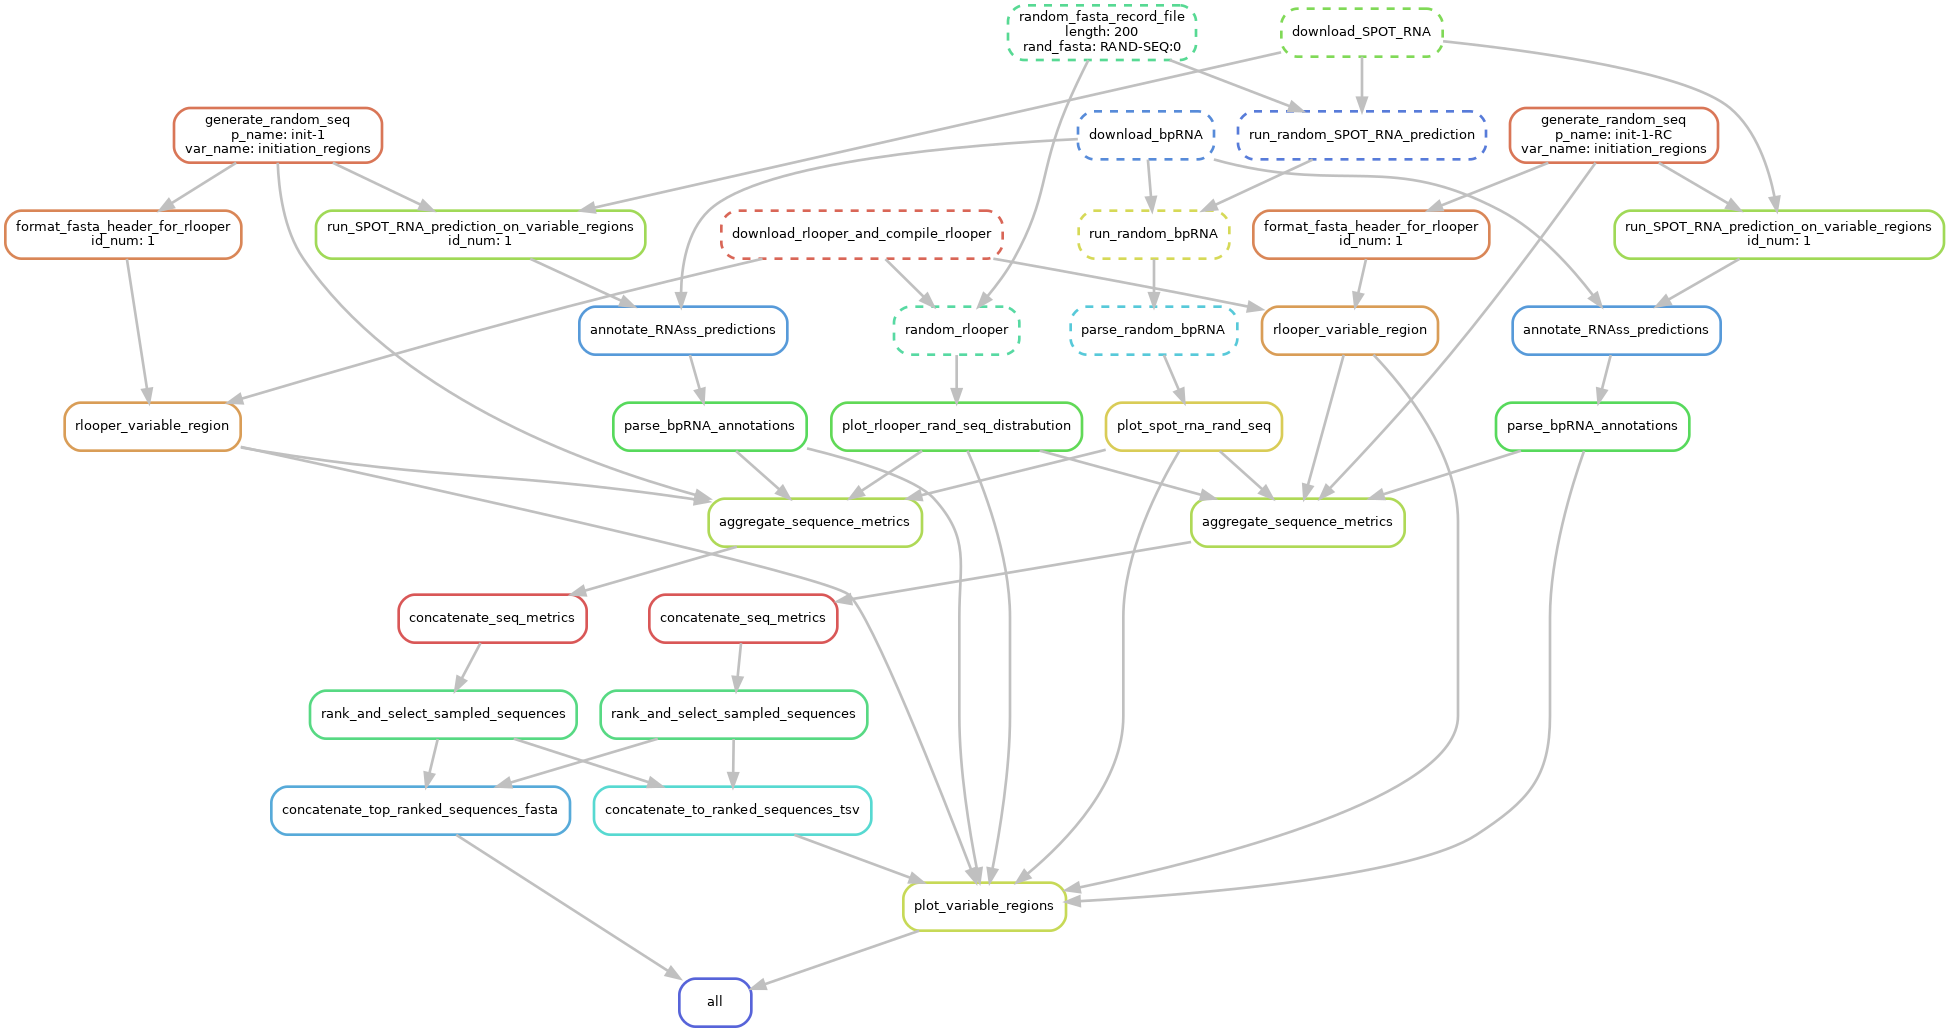
\includegraphics[width=15cm]{images/misc/dag.png}
	\centering
	\caption{Visualization of insert calculation workflow.}
\end{figure}

\subsection{Initial R-looper expectation calculations}


\begin{figure}[H]
	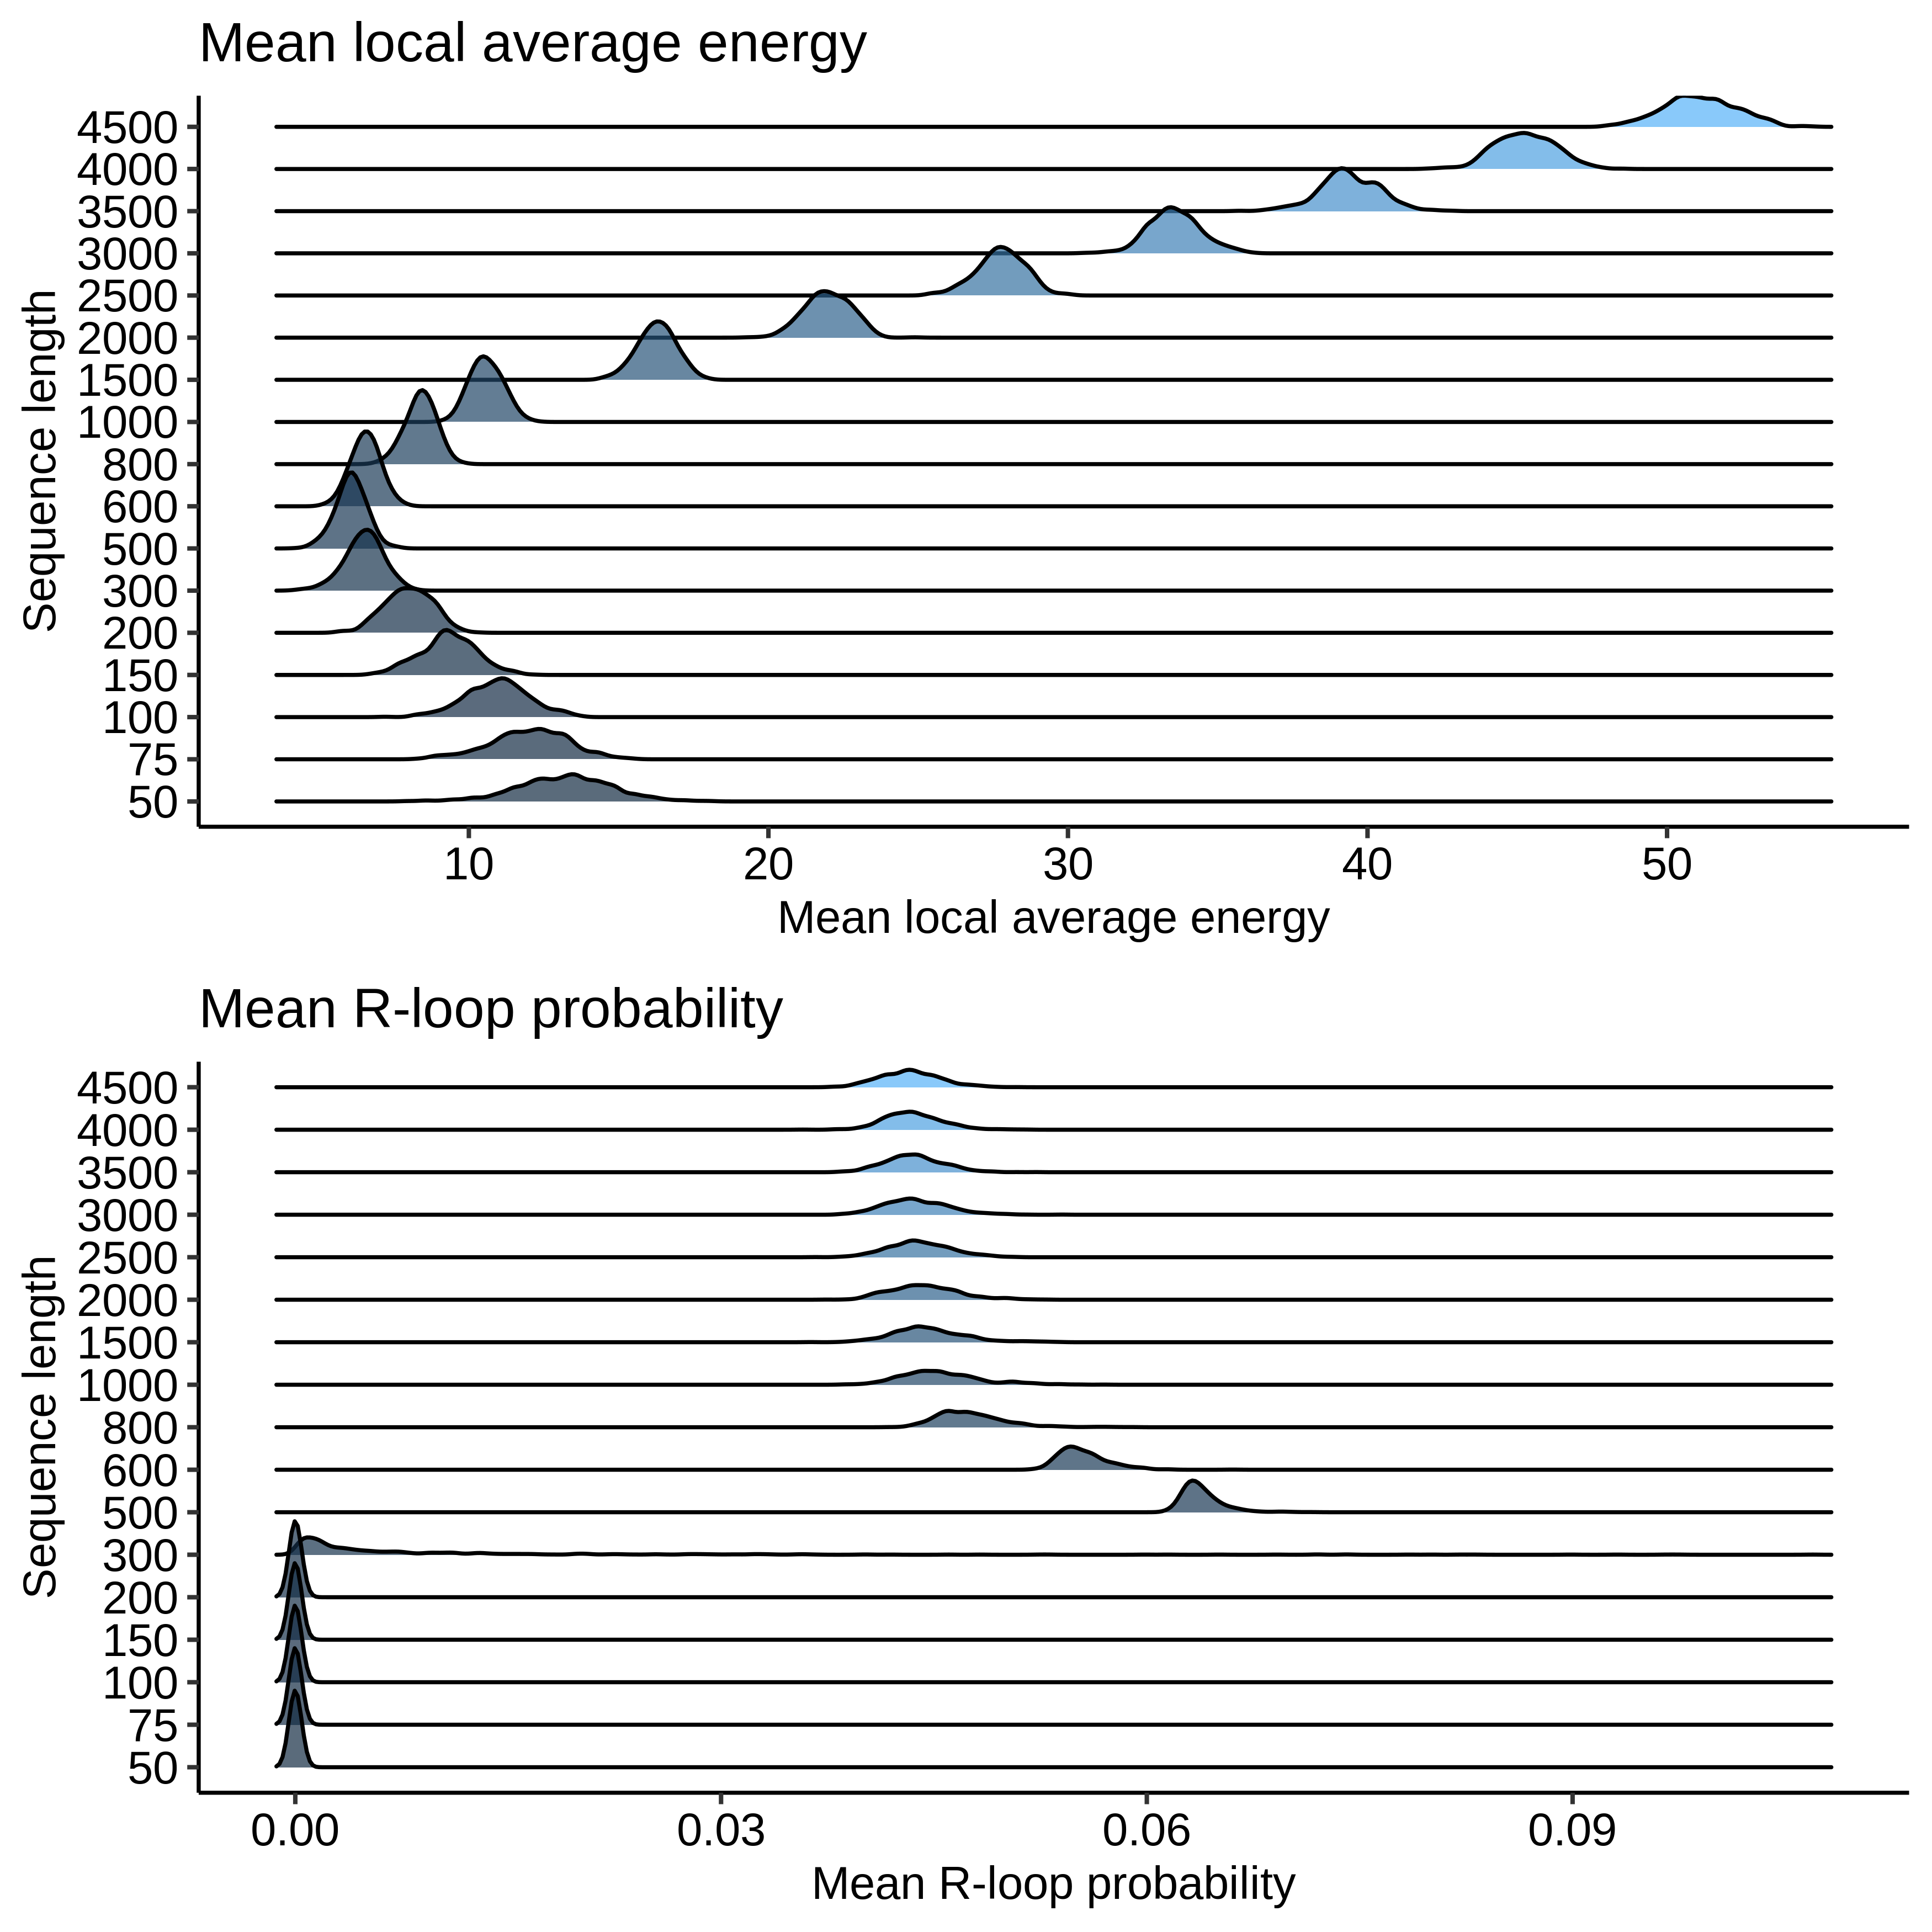
\includegraphics[width=15cm]{images/plots/rand_seq_LAE_dist.png}
	\centering
	\caption{Initial rlooper expectation plots based on completely random sequences of increasing length.}
\end{figure}


\pagebreak

\bibliography{refs/refs.bib}

\end{document}
